% !TeX program = xelatex

\chapter{Ereignisse und Auswertung der Modelle und Algorithmen}
\label{cha:events_and_evaluation}

\section{Trainingsdaten}
Die Bewertung der einzelnen Metriken ist nicht trivial, da die synthetischen Daten nicht nur ähnlich, sondern nicht identisch zu den realen Daten sein sollen. Während bei den meisten Metriken hauptsächlich auf die Übereinstimmung der Daten geschaut wird, oder wie stark deren Verteilungen übereinstimmen, so ist dieser Wert wenig aussagekräftig.
Abweichungen, Werte die nicht in die normale Verteilung passen und andere Abweichungen sind gewollt und dürfen nicht als schlecht bewertet werden.
Visuell lässt sich leicht ein Unterschied zwischen den Daten erkennen, auch kann eingeschätzt werden in wie weit die Daten dem gleichen Muster folgen (siehe Abbildung \ref{fig:real_vs_synth}), nur ist dies kein klassifizierbares Maß.



\begin{figure}[ht]
    \centering
    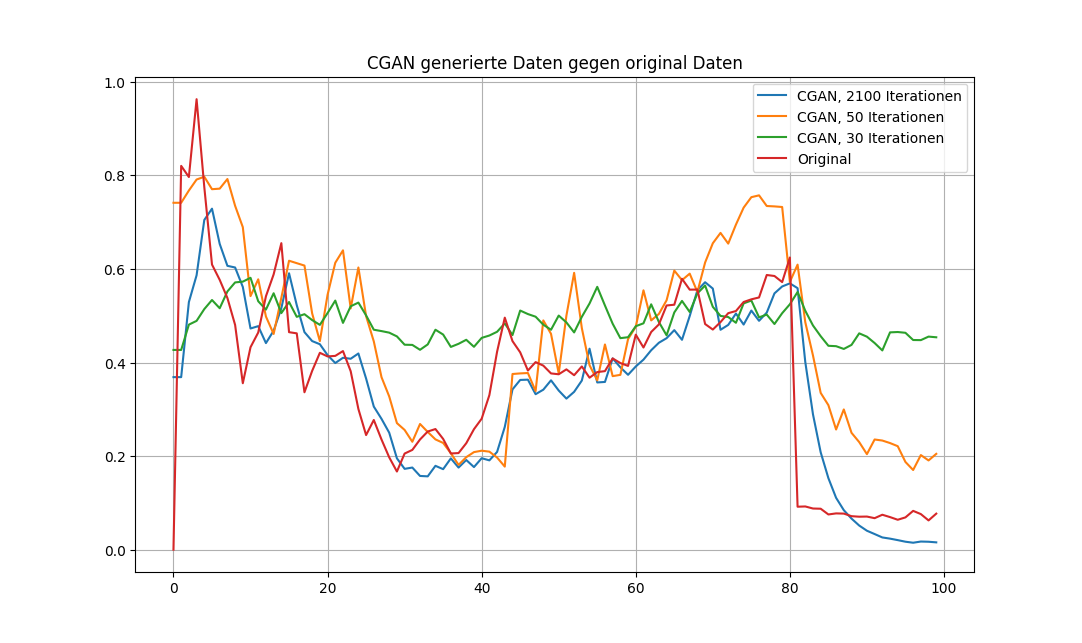
\includegraphics[width=0.8\textwidth]{includes/figures/real_vs_synth.png}
    \caption{Vergleich von realen und synthetischen Daten}
    \label{fig:real_vs_synth}
\end{figure}


\begin{table}[ht]
    \centering
    \caption{Autokorrelation der Datensätze}
    \begin{tabular}{ll}
        \toprule
        \textbf{Dataset Name}   & \textbf{Auto-correlation Coefficient} \\
        \midrule
        weather\_normalized     & 0.7531247393640502                    \\
        stockdata\_normalized   & 0.8705377400789976                    \\
        electricity\_normalized & 0.9213733429685765                    \\
        corona\_normalized      & 0.9705517108865852                    \\
        sinus                   & 0.992051245850721                     \\
        \bottomrule
    \end{tabular}
    \label{tab:autocorrelation_coefficients}
\end{table}


Um die Modelle und Algorithmen später vernünftig zu testen und vergleichen zu können, wurden sie mit 5 verschiedenen Trainingsdaten trainiert.
Diese besitzen jeweils unterschiedliche Komplexität, welche hier durch ihre Autokorrelationswerte angeben und in Tabelle \ref{tab:autocorrelation_coefficients} zu finden ist, und sollen so die Stärken und Schwächen der einzelnen Algorithmen aufzeigen.
Die wohl am einfachten zu erlernenden Daten sind Sinus Kurven. Diese sind leicht zu erlernen und können mit wenigen Parametern beschrieben werden.
In Abbildung \ref{fig:sinus_data} sind die Daten zu sehen.

\begin{figure}[ht]
    \centering
    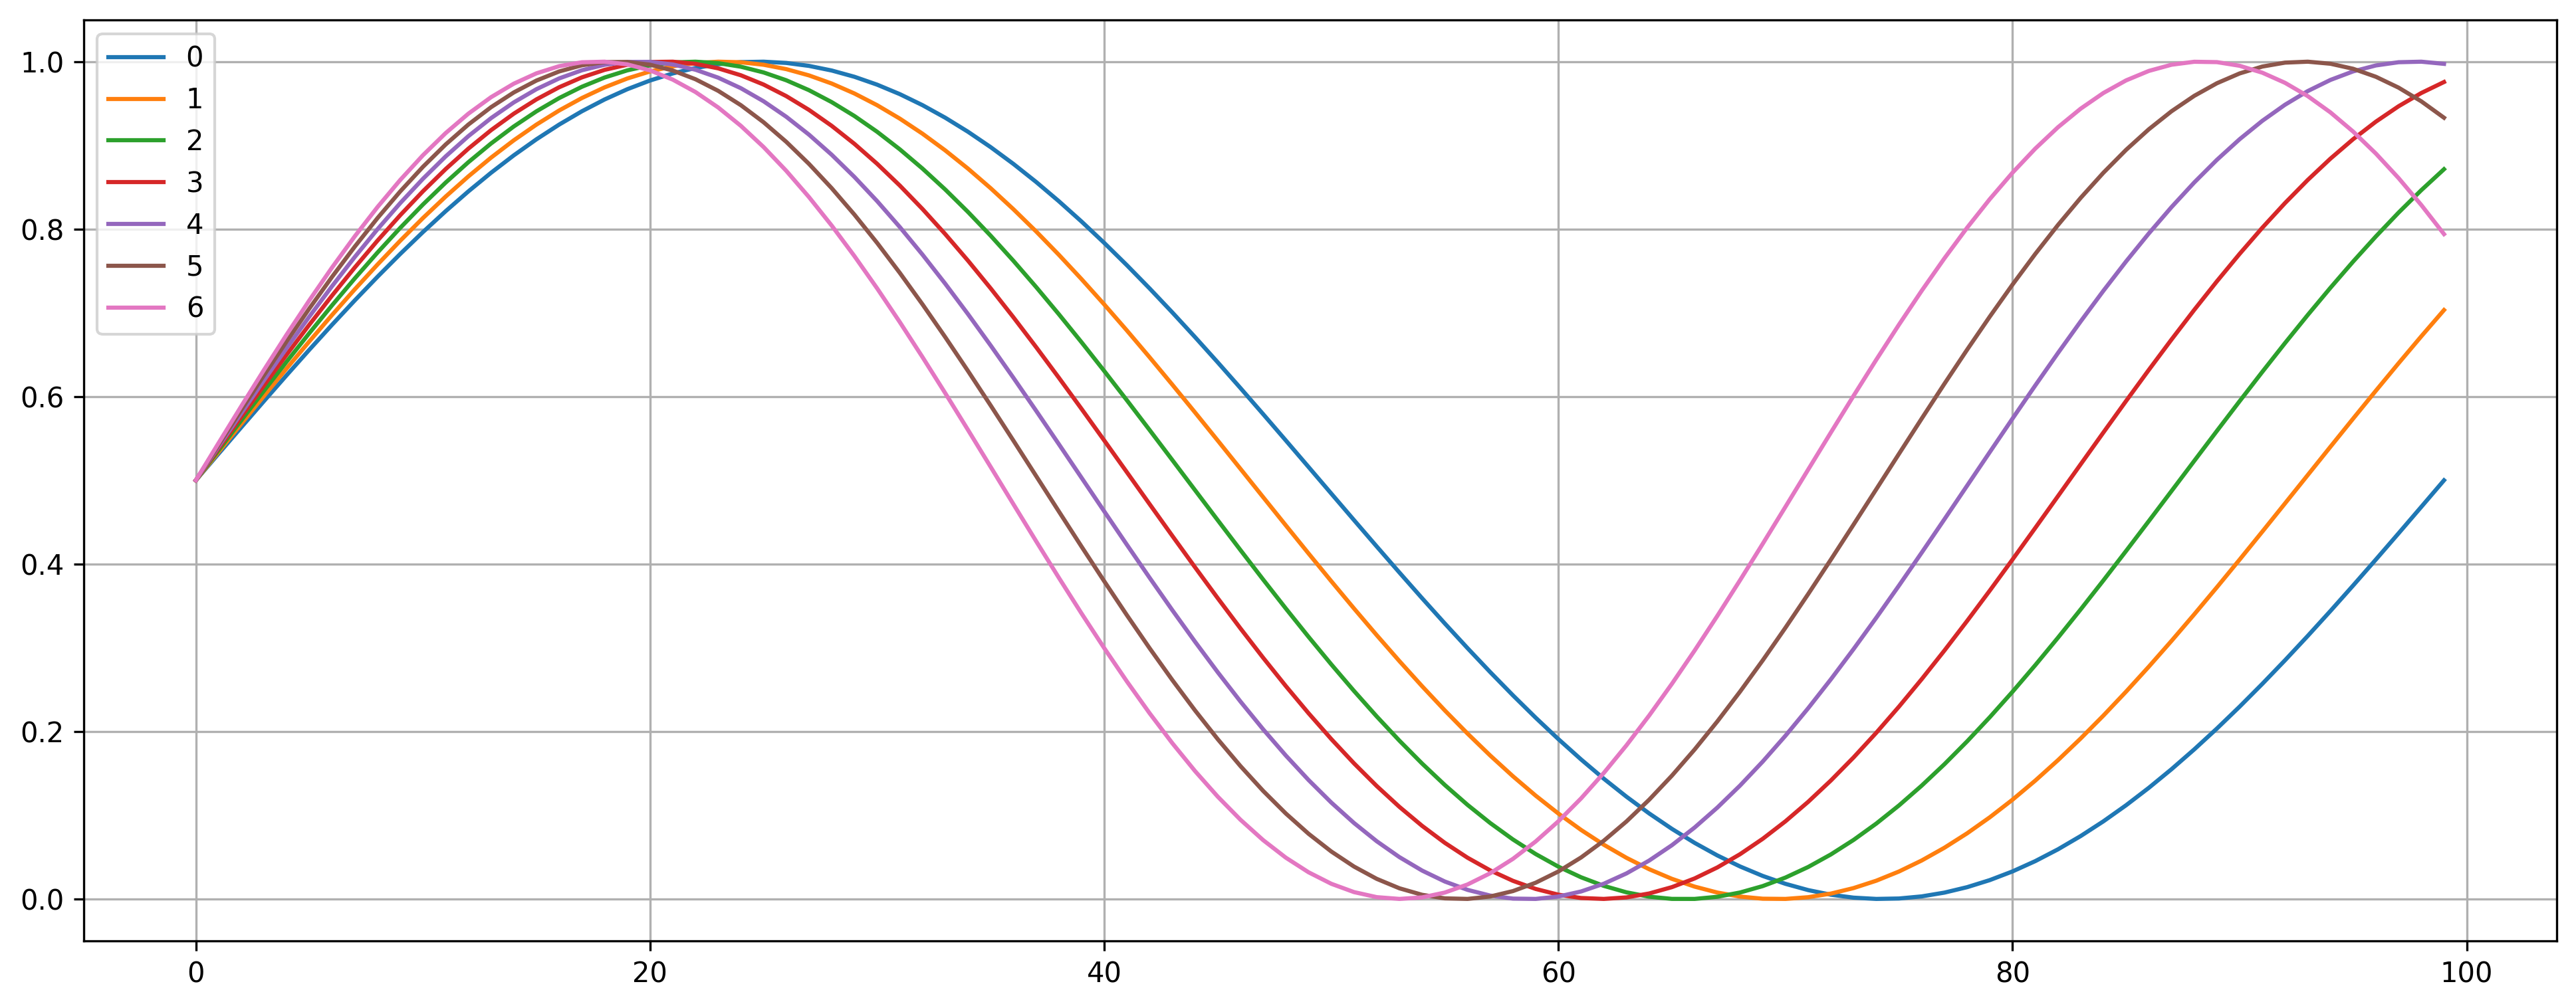
\includegraphics[width=1\textwidth]{includes/figures/graphs/sinus.png}
    \caption{Sinus Kurven als Testdaten}
    \label{fig:sinus_data}
\end{figure}

Die genutzten Corona Daten zeigen den Anstieg zum Beginn der Pandemie, und sind daher wenig komplex. Diese stammen von \cite{covid19g12:online} und sind in Abbildung \ref{fig:covid_data} zu sehen.

\begin{figure}[ht]
    \centering
    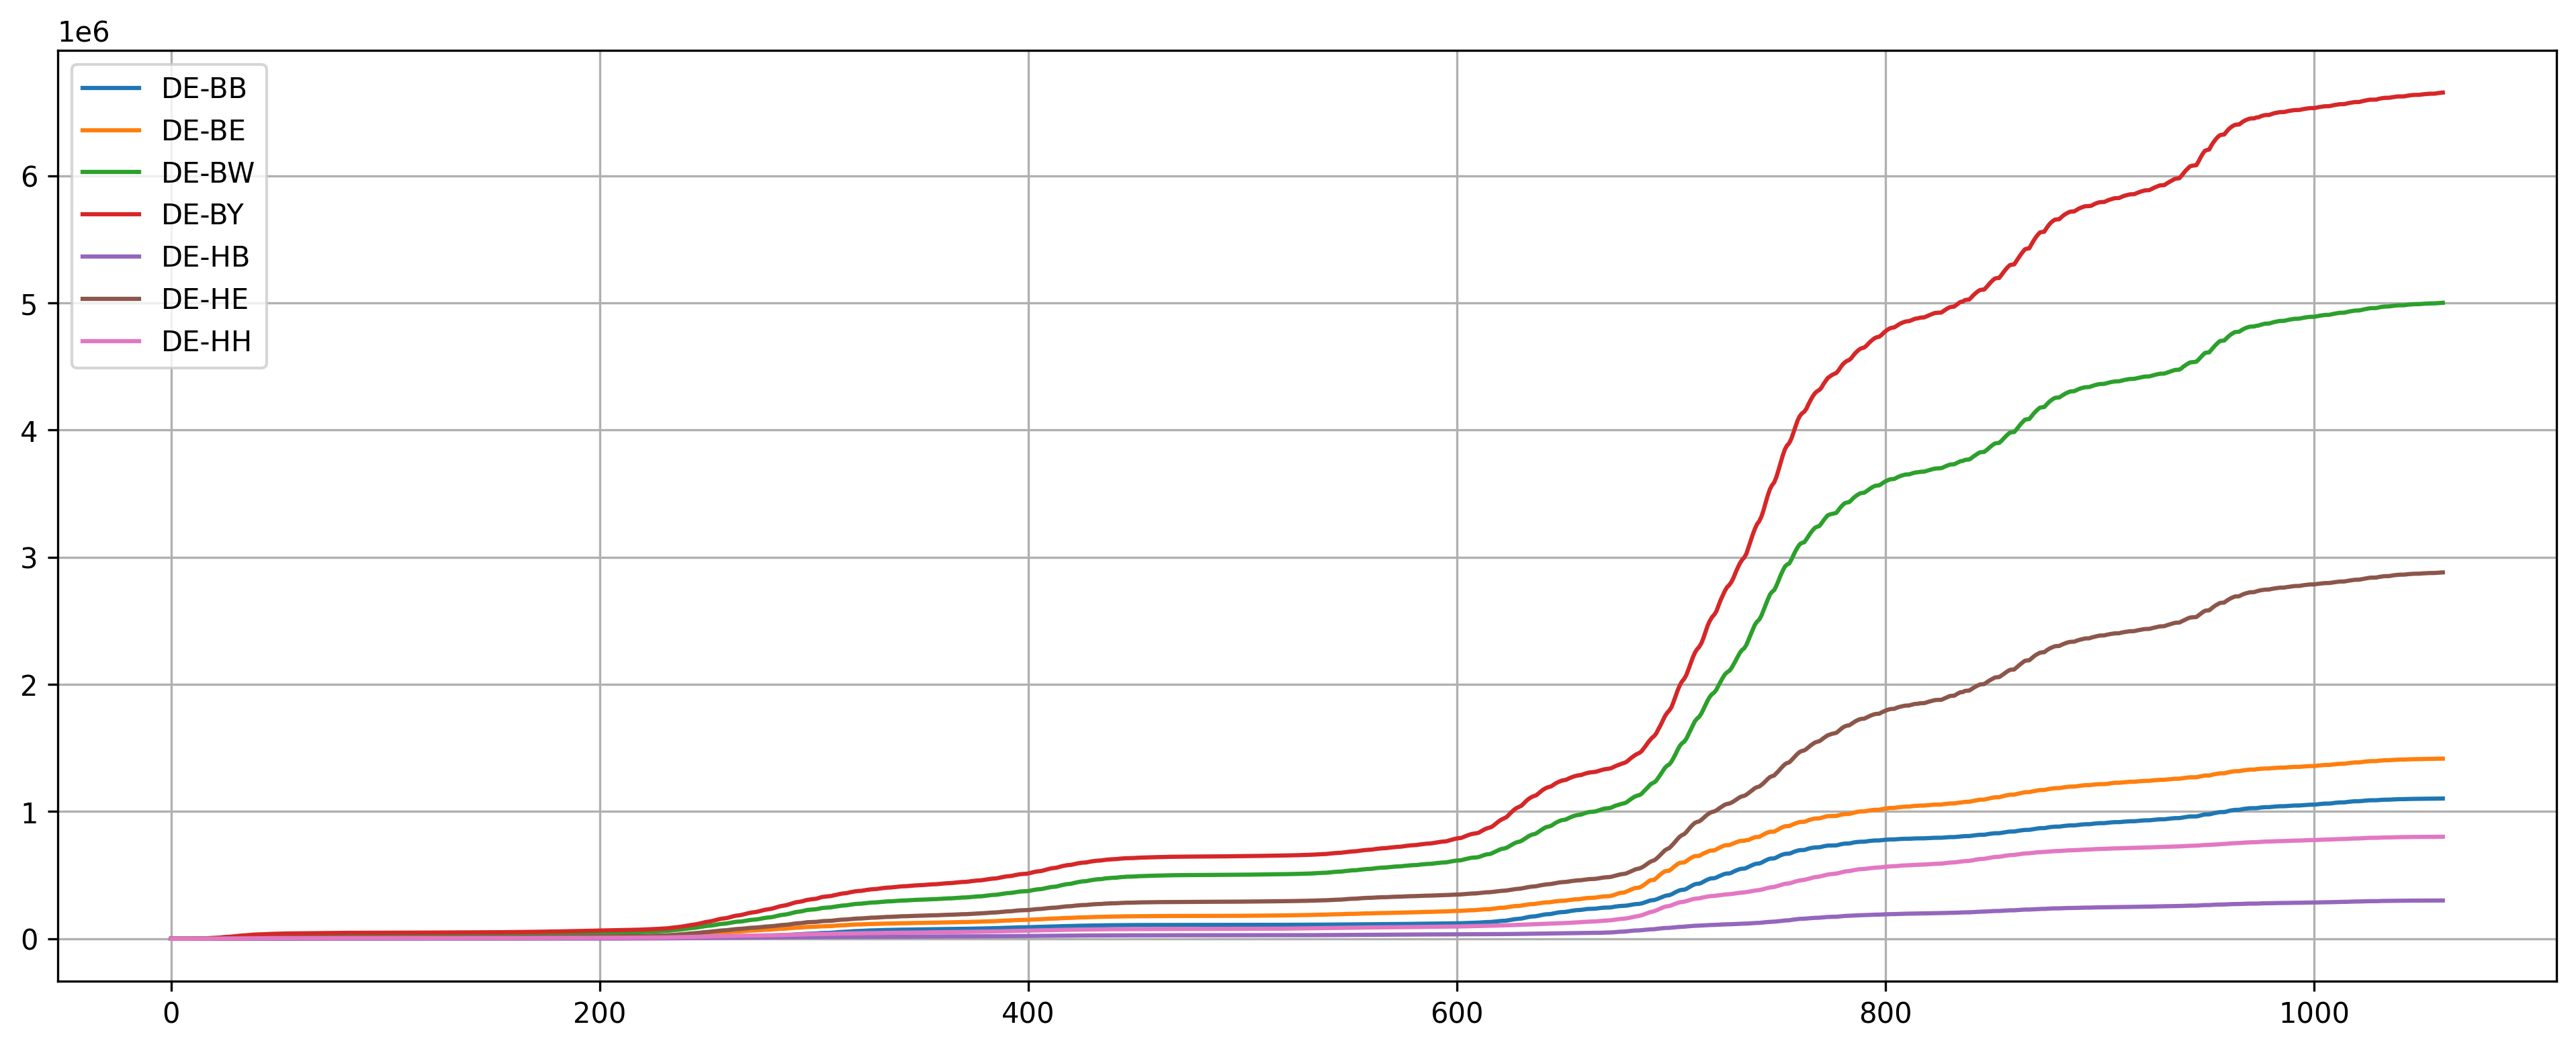
\includegraphics[width=1\textwidth]{includes/figures/graphs/corona_test_cases.png}
    \caption{Infektionszahlen einiger Bundesländer zu Beginn der Pandemie als Testdaten}
    \label{fig:corona_data}
\end{figure}

Etwas komplexer sind die Daten über den Stromverbrauch von unterschiedlichen Verbrauchern über mehrere Tage hinweg, der genutzte Datensatz misst die Werte für verschiedenen Haushalte über etwas mehr als 30 Tage im stündlichen Takt. Sie stammen von \cite{longterm99:online} und hatten leider wenige Information über die Art der Daten.
Hier treten periodische Muster auf, welche aber nicht so einfach zu erlernen sind wie die Sinus Kurven und damit eine größere Herausforderung darstellen.
Auch sind hier Außreißer und andere Abweichungen von der Norm zu erwarten. Die Daten sind in Abbildung \ref{fig:electric_data} zu sehen.

\begin{figure}[ht]
    \centering
    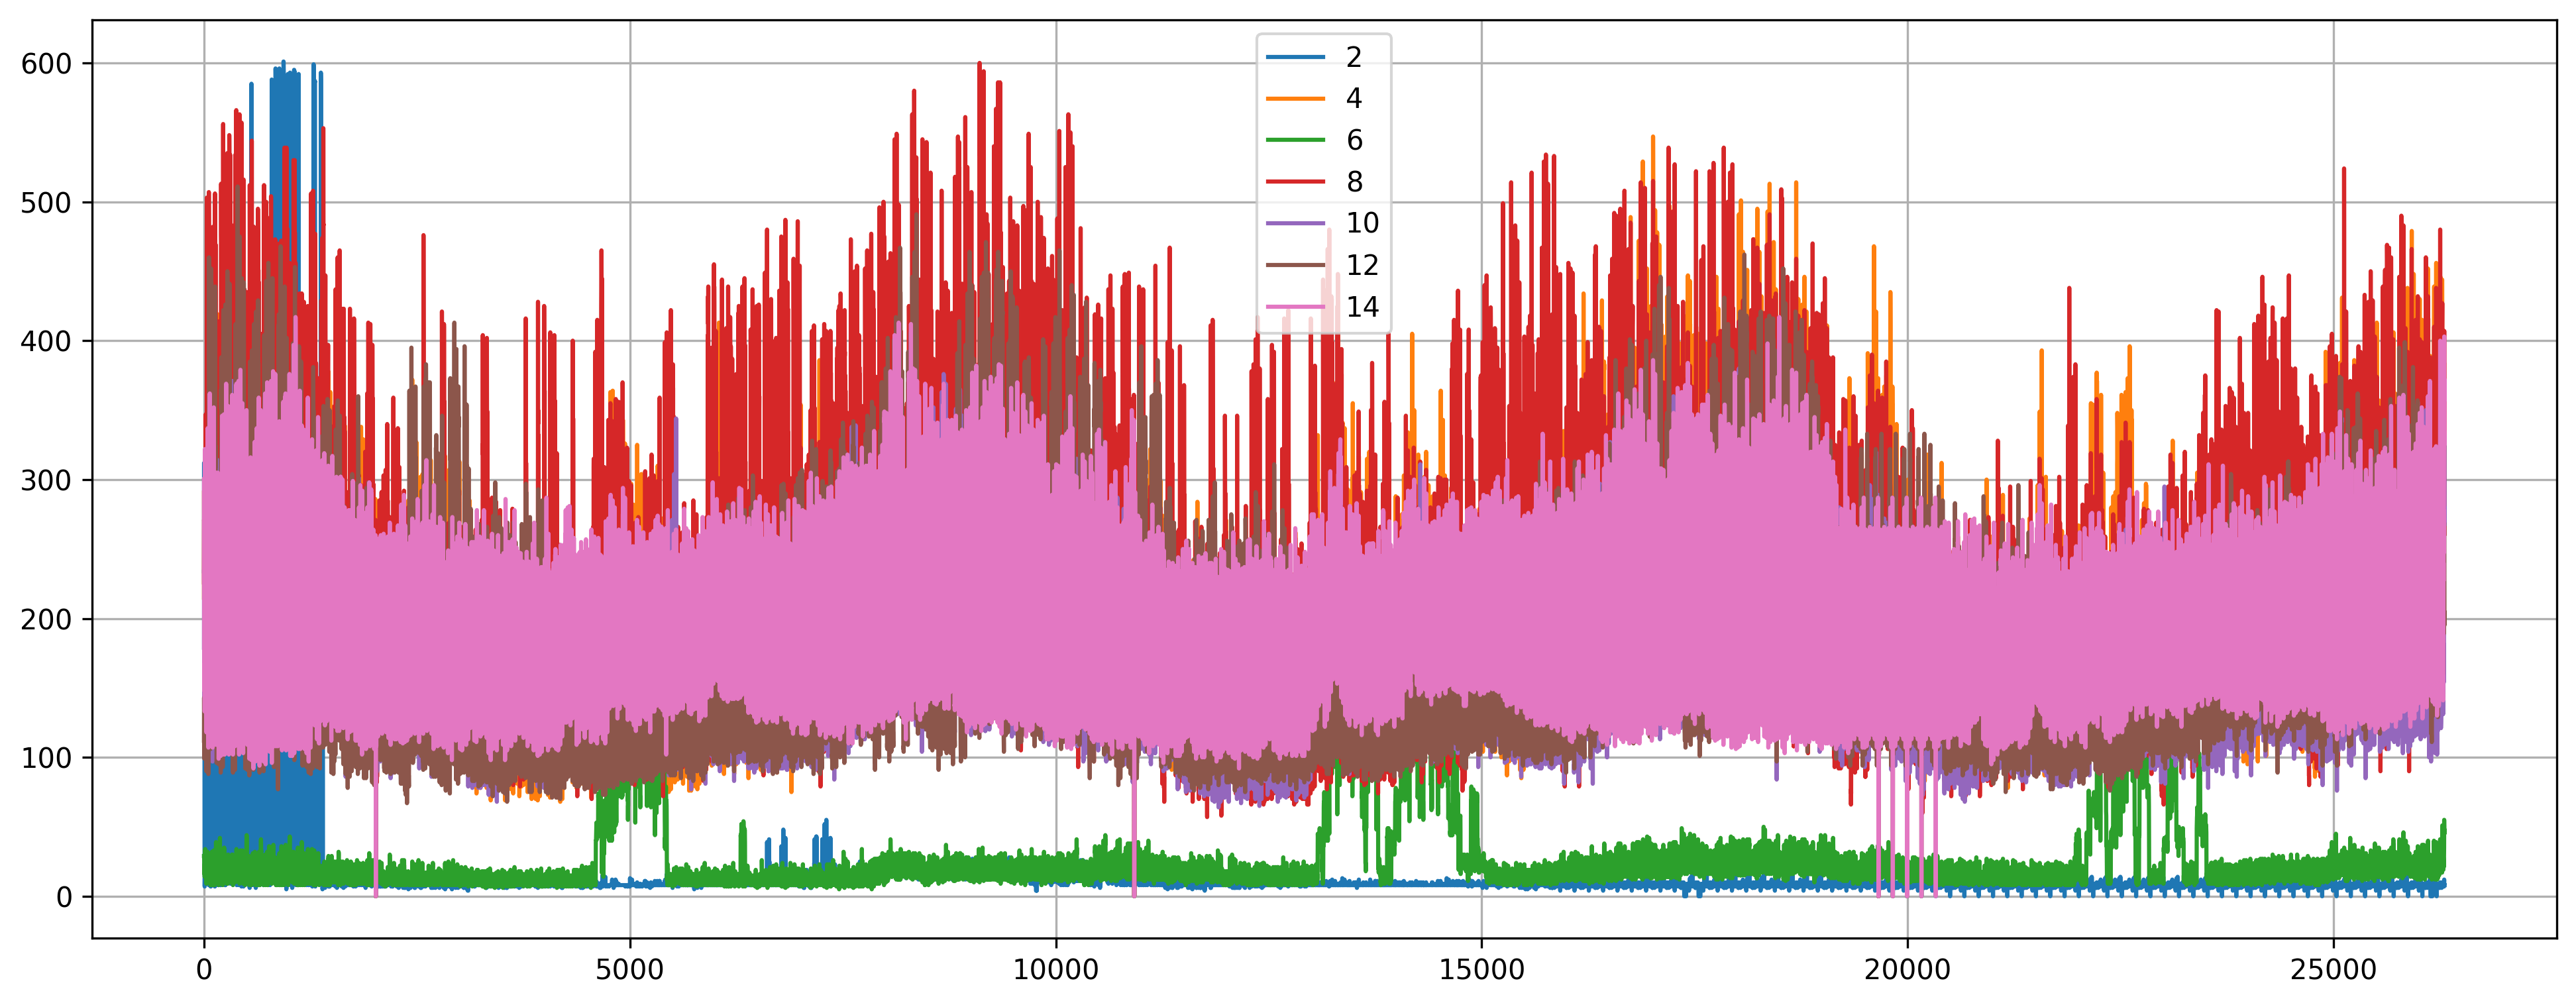
\includegraphics[width=1\textwidth]{includes/figures/graphs/electricity.png}
    \caption{Elektrizitätsverbrauch als Testdaten}
    \label{fig:electric_data}
\end{figure}



Sehr interessant sind auch Aktiendaten. Diese sind sehr komplex, nicht zwangsläufig periodisch und besitzen viele Abweichungen von der Norm. Sie sind deutlich komplexer zu erlernen, da sie keinen direktem Muster folgen.
Die Daten sind in Abbildung \ref{fig:stock_data} zu sehen und wurden über Yahoo Finanzen\footnote{https://de.finance.yahoo.com/} erworben. Da es sich um die selber Aktie und verschieden Werte handelt, wie beispielsweise deren höchsten, niedrigersten oder durschnittlichen Preis, sind die Daten sehr ähnlich, aber nicht identisch.

\begin{figure}[ht]
    \centering
    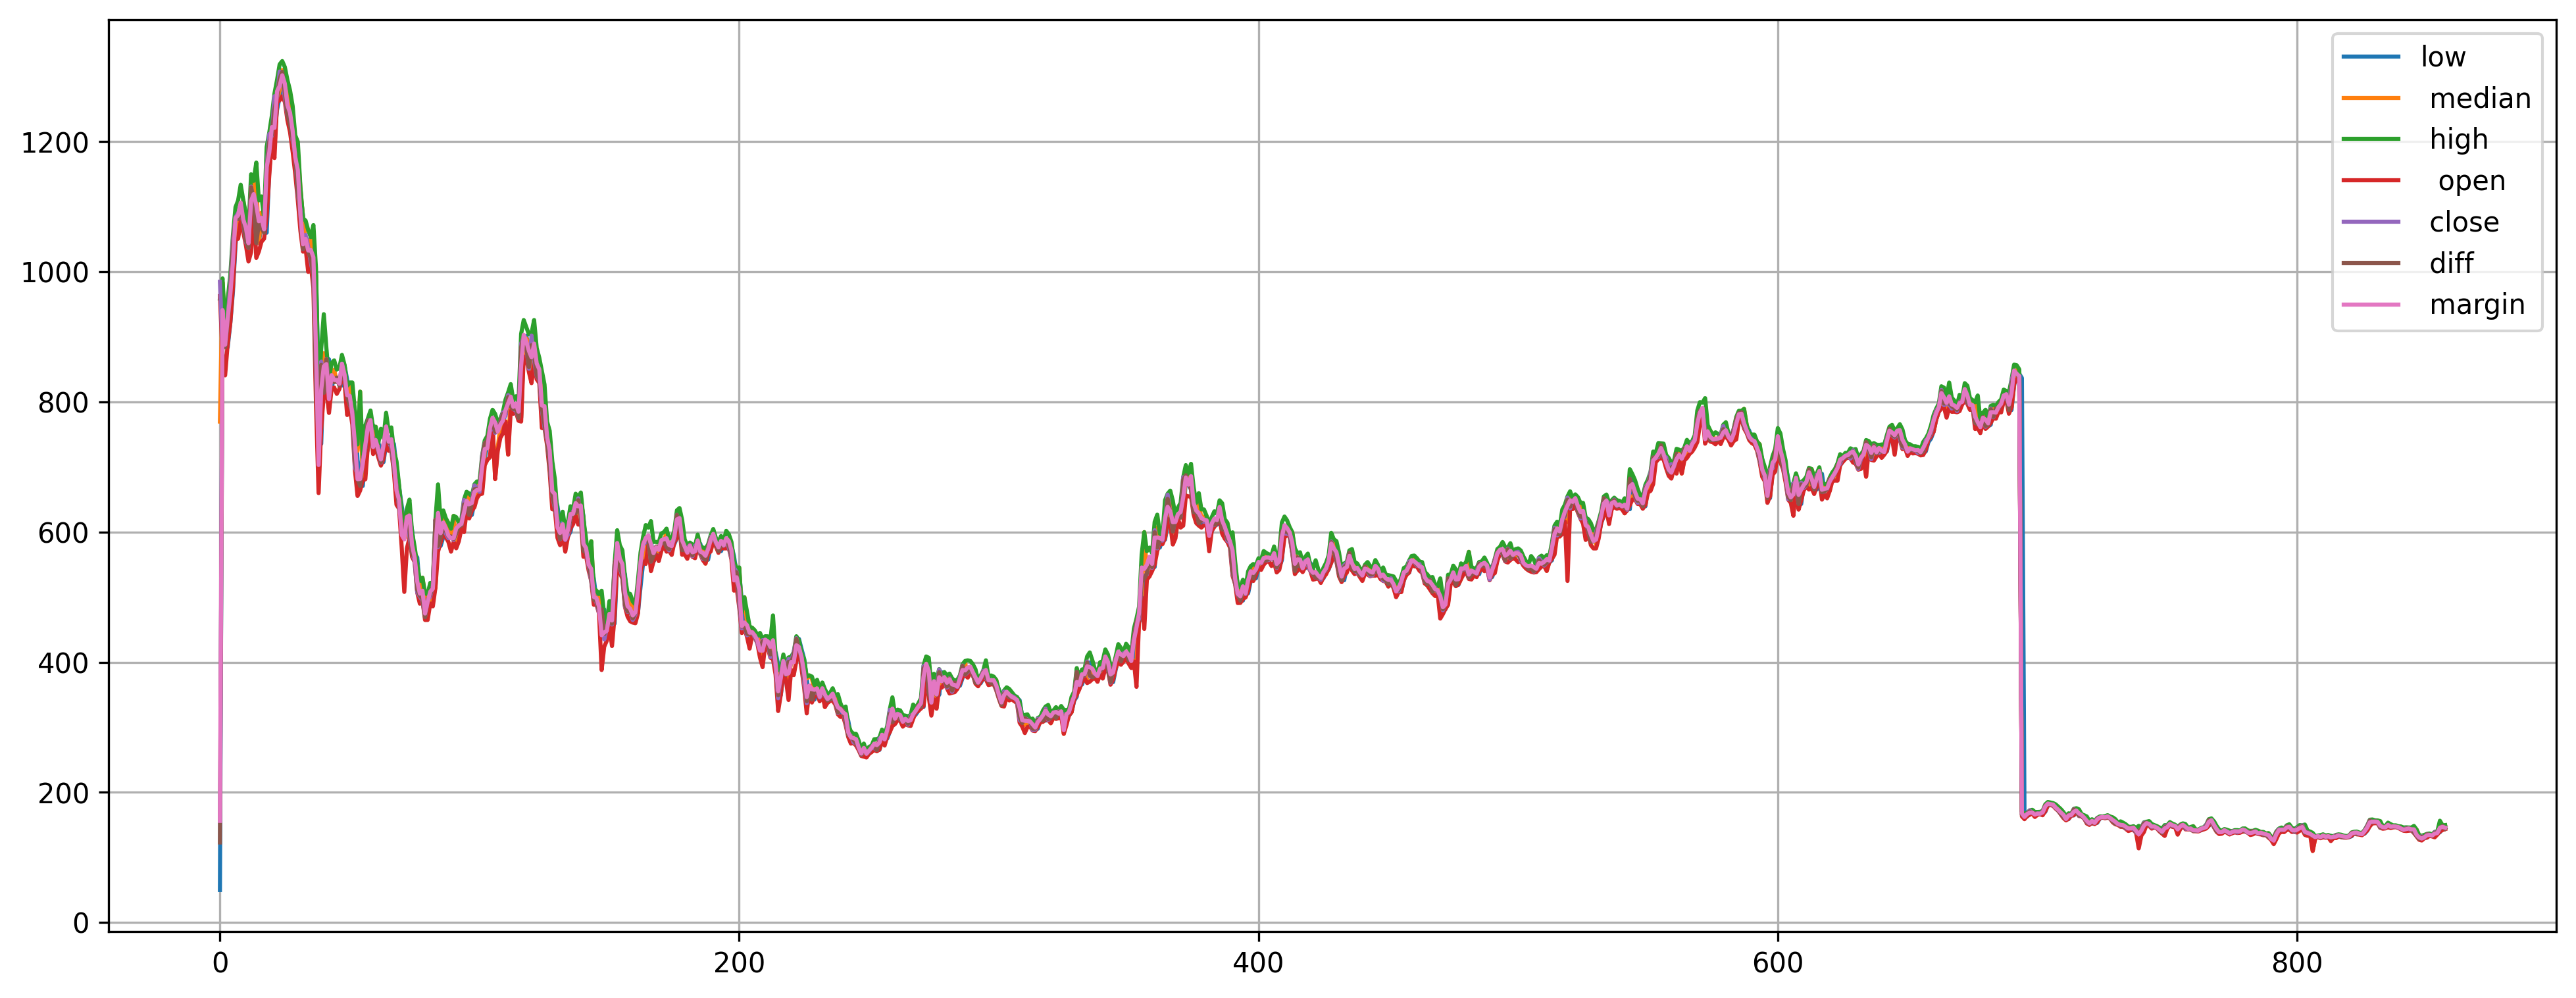
\includegraphics[width=1\textwidth]{includes/figures/graphs/stockdata.png}
    \caption{Aktiendaten als Testdaten}
    \label{fig:stock_data}
\end{figure}



Interesannter weise sind die Wetterdaten über einen gewissen Zeitraum am komplexesten. Diese sind Teilweise periodisch, aber auch nicht immer. 
Dazu kommt der Umstand, dass nicht nur Temperaturen, sondern auch Luftdruck und andere Werte mit aufgenommen wurden. Ein Überblick ist in Abbildung \ref{fig:weather_data} zu sehen. Sie stammen auch von \cite{longterm99:online} und es gibt daher 
auch keine weiteren Informationen über die Daten.

\begin{figure}[ht]
    \centering
    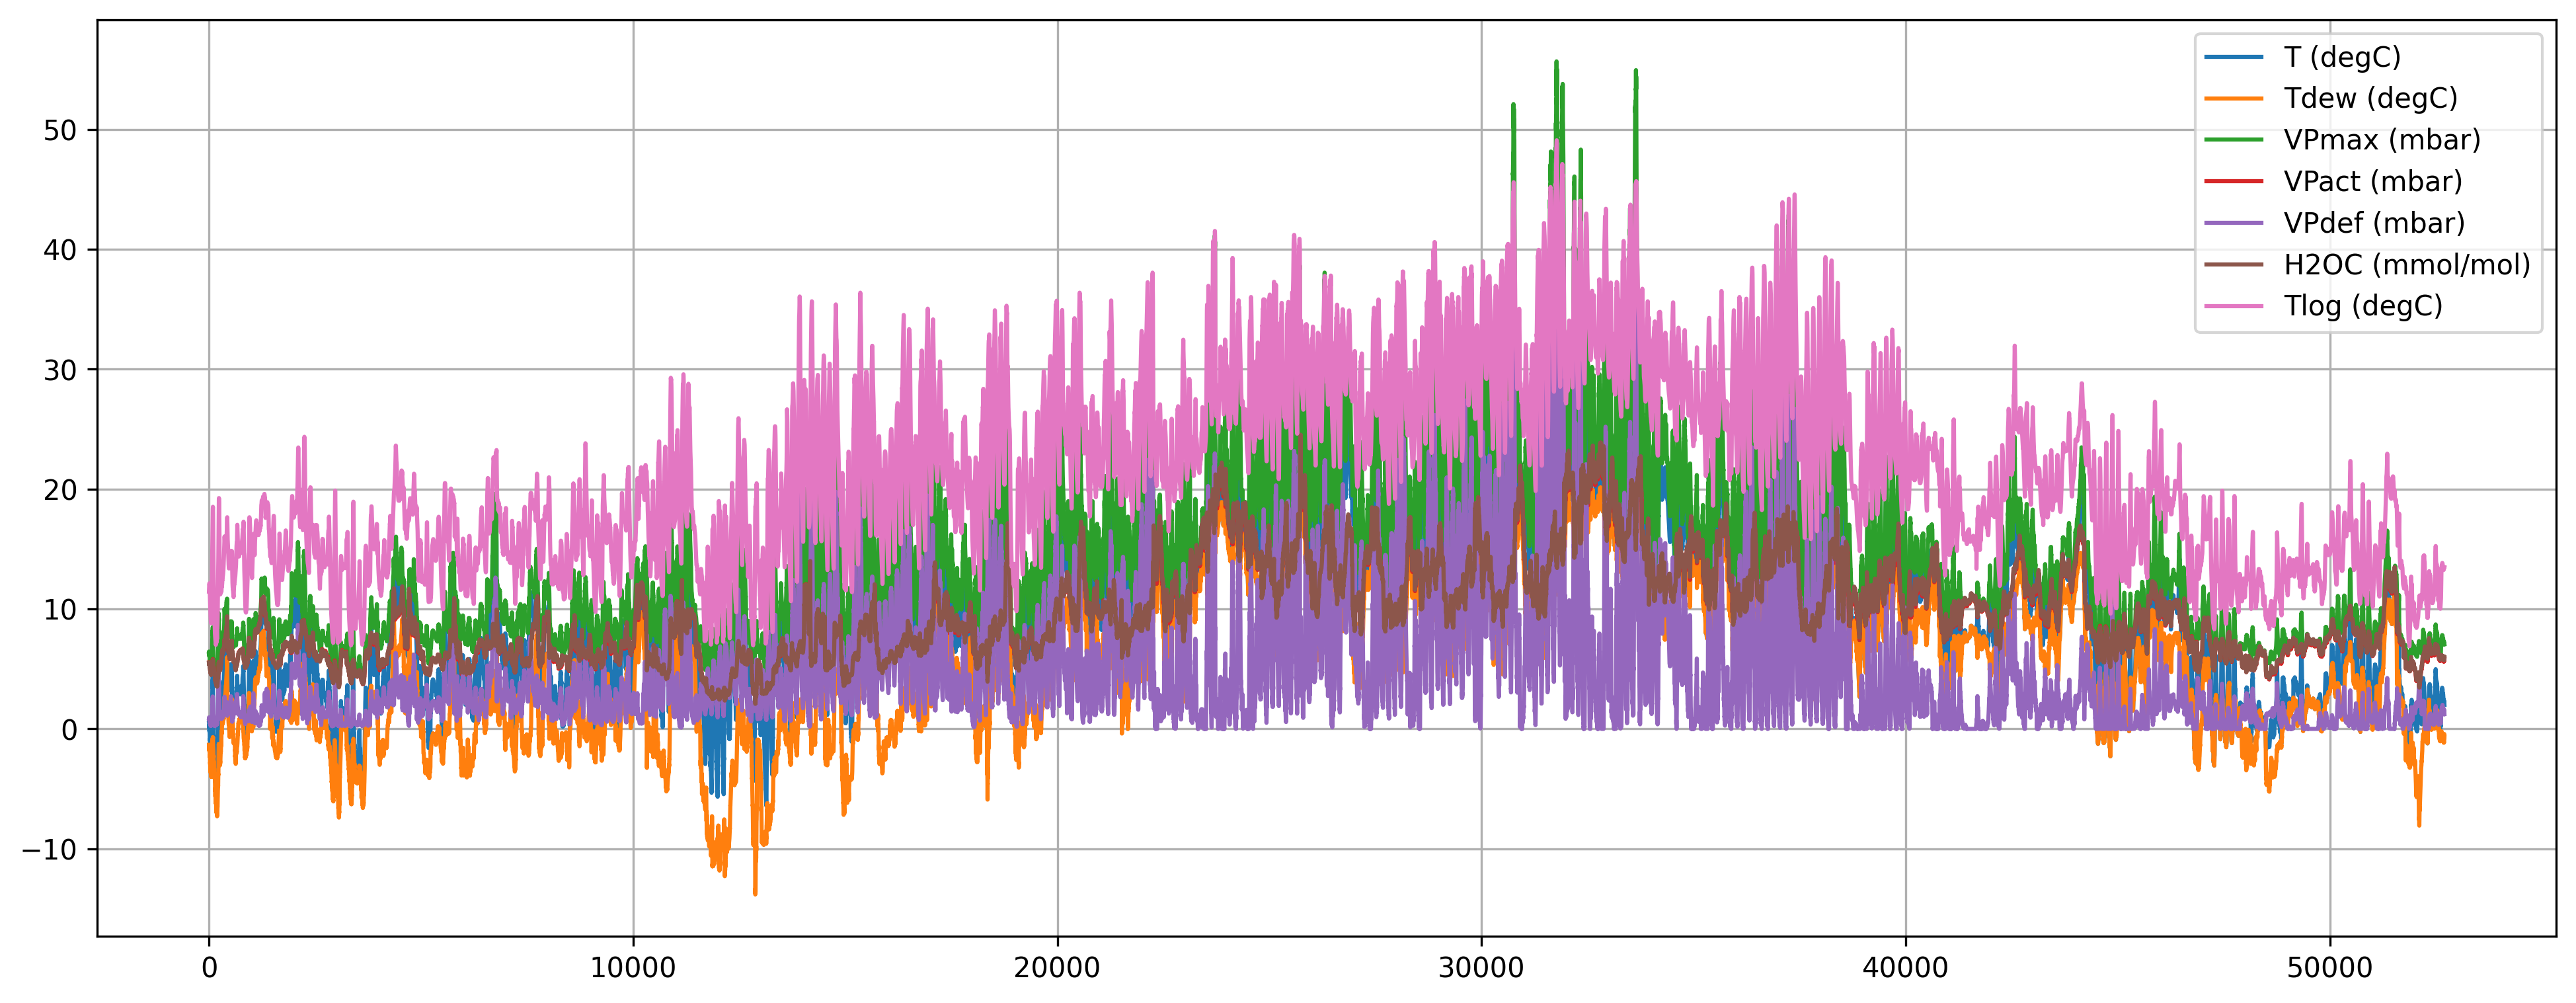
\includegraphics[width=1\textwidth]{includes/figures/graphs/weather.png}
    \caption{Wetterdaten als Testdaten}
    \label{fig:weather_data}
\end{figure}


\section{Vergleich der Algorithmen und Modelle}

\subsection{Performance Metriken der ML Modelle}

Um die Vergleichbarkeit der einzelnen Metriken zu gewährleisten, wurden die realen Daten alle ersteinmal uniformiert. Dies bedeutet, dass die Daten auf einen Wertebereich von 0 bis 1 skaliert wurden und auf die gleiche Anzahl an Elementen je Zeitreihe gebracht wurden.
Somit lässt dich der Vorverarbeitungsschritt entfernen und die Modelle können direkt auf den Daten trainieren.

Grundsätzlich sind die Trainingszeiten der generativen Modelle stark unterschiedlich. Modelle aus der tsgm Bibliothek \cite{nikitin2023tsgm} sind deutlich deutlich langsamer als die nativen keras Modelle, welche selber implementiert wurden.
Da aber die tsgm Modelle bei weitem komplexer sind und bereits nutzbare Ergebnisse mit wenigeren Iterationen liefern, wurde hier die Zahl der Iterationen reduziert, um die Laufzeit zu verkürzen.
Der Test wurde nur mit wenigen Iterationen durchgeführt, da hier am entscheidensten die Menge an Daten zum Training relevant war.
Um die Einflüsse anderer Programme auf dem System zu eliminieren oder wenigstens zu minimieren wurde der Test in einen eigens hierfür erstellten Docker Containern durchgeführt. Dieser Container wurde mit 2 \ac{CPU} Kernen und 8 \ac{GB} \ac{RAM} ausgestattet.

\begin{figure}[ht]
    \centering
    \begin{minipage}{0.6\textwidth}
        \centering
        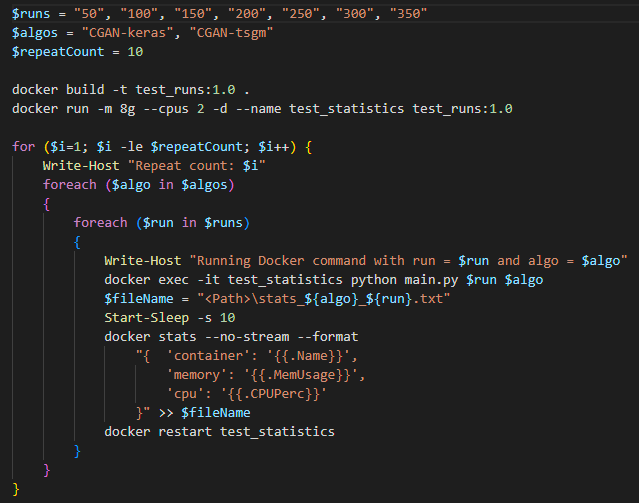
\includegraphics[width=\textwidth]{includes/figures/code/powershell_for_testing.png}
        \caption{PowerShell Script zum Testen der Modelle in einem Docker Container}
        \label{fig:test_run_powershell}
    \end{minipage}\hfill
    \begin{minipage}{0.38\textwidth}
        \centering
        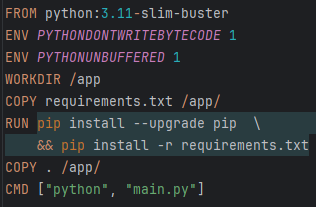
\includegraphics[width=\textwidth]{includes/figures/code/Dockerfile_for_testing.png}
        \caption{Dockerfile zum Erstellen des Docker Containers}
        \label{fig:test_run_dockerfile}
    \end{minipage}
\end{figure}

Da sowohl die tsgm Bibliothek als auch selber eine Implementierung der \ac{CGAN} Architektur erstellt wurde, bat es sich an diese als Vergleich zu nutzen. Wie in Abbildung \ref{fig:test_run_powershell} zu sehen ist, wird der Docker Container über ein Powershell Script gebaut, startet das Python Script, speichert alle notwendigen Metriken und startet den Container neu.
Dies sorgt dafür, dass alle gesammelten Resourcen wieder freigegeben werden und somit ein klares Bild über die realen Anforderungen des Modells entstehen. Damit fremde Einflüssen auf die Messungen minimiert werden, wurde der Test 6 mal wiederholt und der Durschnitt gebildet
Die Ergebnisse sind in Abbildung \ref{fig:compare_run_time_iterations} zu sehen.
Es wir klar, dass die tsgm Implementierung deutlich länger braucht als die des nativen keras Modells.
Dies lässt sich auf mehrere entscheidende Faktoren zurückzuführen. Die tsgm Bibliothek ist noch sehr neu und, zur Zeit der Implementierung, erst in Version 0.0.4. Auch sind die Architektur der Modelle komplexer, da sie mit deutlich mehr Parametern in mehrer Schichten trainieren.


\begin{figure}[ht]
    \centering
    \begin{minipage}{0.5\textwidth}
        \centering
        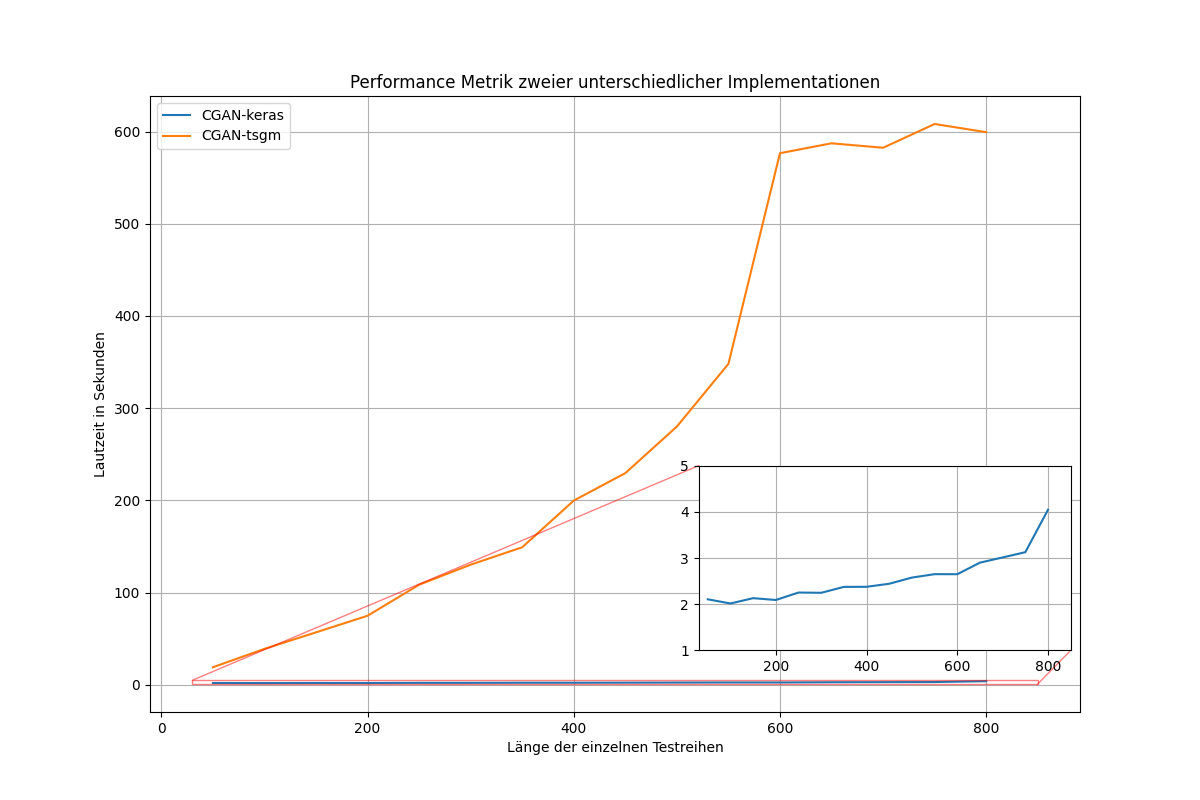
\includegraphics[width=\textwidth]{includes/figures/compare_run_time_iterations.png}
        \caption{Laufzeit des nativen CGAN Modells im Vergleich zur tsgm Implementierung in Abhängigkeit der Länge der Zeitreihen}
        \label{fig:compare_run_time_iterations}
    \end{minipage}\hfill
    \begin{minipage}{0.5\textwidth}
        \centering
        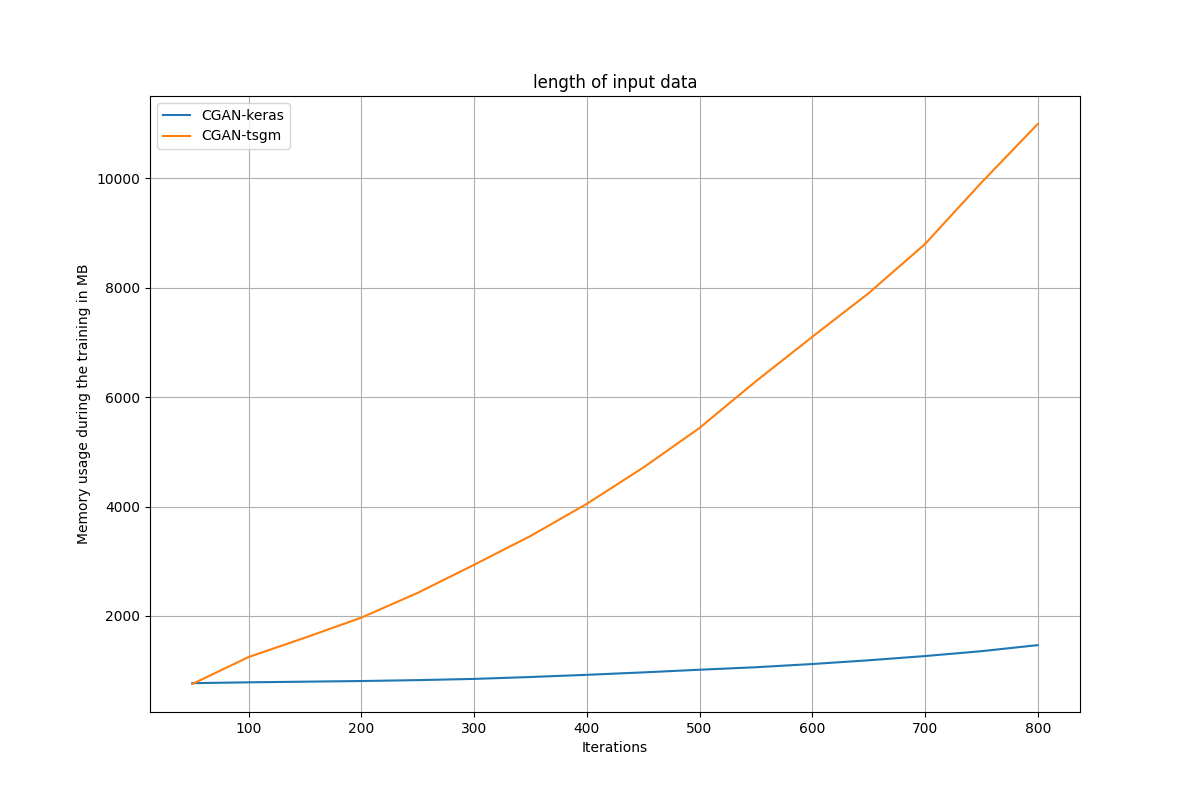
\includegraphics[width=\textwidth]{includes/figures/ram_usage_tsgm_vs_keras.png}
        \caption{RAM Auslastung des nativen CGAN Modells im Vergleich zur tsgm Implementierung in Abhängigkeit der Länge der Zeitreihen}
        \label{fig:compare_ram_usage}
    \end{minipage}
\end{figure}


Dennoch ist der nur sehr geringe Anstieg der Laufzeiten des Keras Modells sehr beeindruckend. Keras hat einen minimalen Anstieg, während der Anstieg der tsgm Modelle linear zur Anzahl der Iterationen ist.
Da der \ac{RAM} Verbrauch der tsgm Modelle sehr hoch war, wurde dieser auch gemessen. Hier ist auch wieder der Docker Container hilfreich, da die Isolation der Container dafür sorgt, dass der Verbrauch nicht durch andere Programme beeinflusst wird.
Wie in Abbildung \ref{fig:compare_ram_usage} zu sehen ist, ist selbst bei kleinen Modellen der \ac{RAM} Verbrauch der tsgm Modelle deutlich höher als der der nativen Modelle. Daher ist besonderst für diese eine vernünftige Vorverarbeitung wichtig,
da sonst weder die Laufzeit noch die Hardware Anforderungen von normalen Computern akzeptabel bzw ausreichen sind.


In Abbildung \ref{fig:train_time_compared} ist noch einmal der Verlauf aller getesteten Modelle zu sehen. Hier ist deutlich zu erkennen, dass die meisten tsgm Modelle deutlich mehr Zeit benötigen als die nativen Modelle.
\begin{figure}[ht]
    \centering
    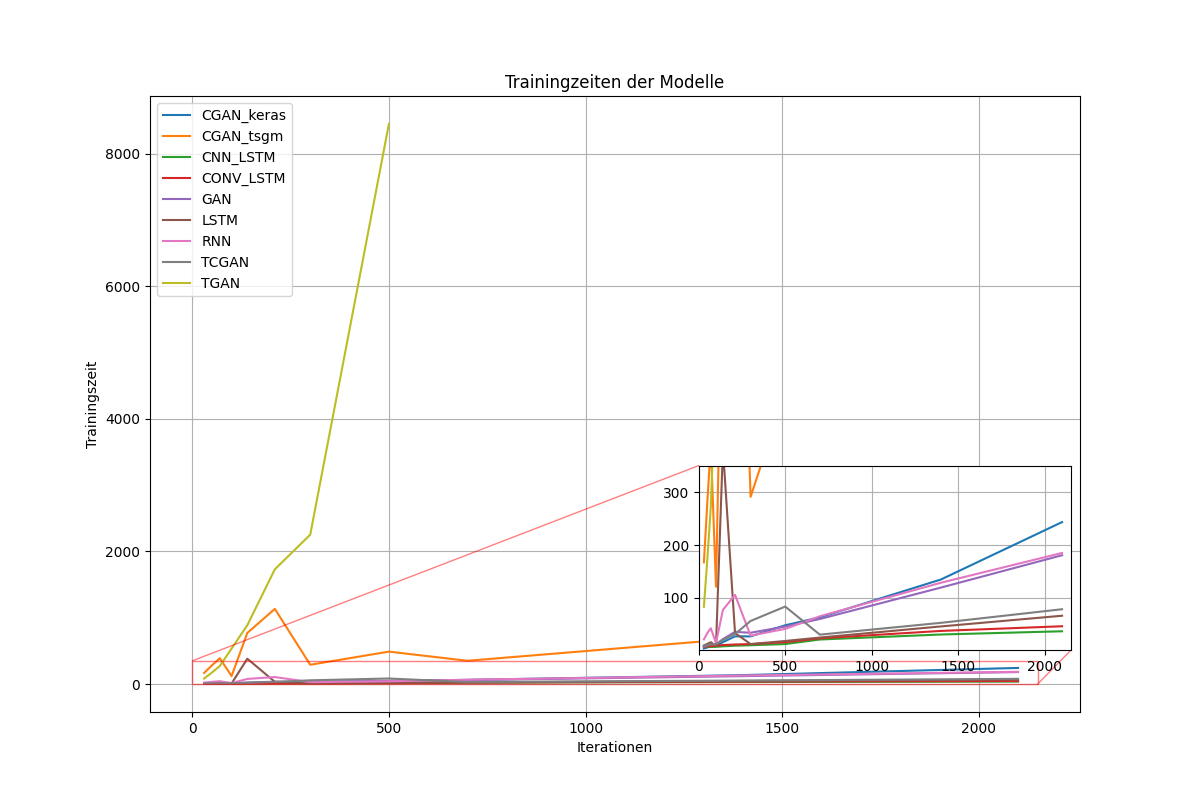
\includegraphics[width=1\textwidth]{includes/figures/graphs/train_time_compared.png}
    \caption{Laufzeit der einzelnen Modelle im Vergleich zur Anzahl der Iterationen}
    \label{fig:train_time_compared}
\end{figure}



\subsection{Performance Metriken der TSA Algorithmen}
Die Trainingszeiten der \ac{TSA} Algorithmen sind deutlich geringer als die der \ac{ML} Modelle, wie in Tabelle \ref{tab:trainingszeiten_tsa} zu sehen ist.
Der Cubic Spline Algorithmus ist hierbei der schnellste, da er nur eine Interpolation durchführt und keine weiteren Berechnungen benötigt.
Schaut man auf die anderen Modelle, so fällt Amira auf, dieser ist weitaus langsamer als die anderen Algorithem.
Dies liegt daran, dass Amira eine sehr komplexe Architektur besitzt und daher deutlich mehr Rechenleistung benötigt.

\begin{table}[ht]
    \centering
    \caption{Trainingszeiten der \ac{TSA} Algorithmen}
    \begin{tabular}{lrr}
        \toprule
        Algorithm & Iteration & Trainingszeit in Sekunden \\
        \midrule
        Amira     & /         & 0.452361                  \\
        Cubic     & /         & 0.004374                  \\
        EMD       & 0         & 0.038583                  \\
        EMD       & 1         & 0.038053                  \\
        EMD       & 2         & 0.040761                  \\
        EMD       & 3         & 0.039456                  \\
        SSA       & 0         & 0.013947                  \\
        SSA       & 1         & 0.014150                  \\
        SSA       & 2         & 0.012575                  \\
        SSA       & 3         & 0.012223                  \\
        \bottomrule
    \end{tabular}
    \label{tab:trainingszeiten_tsa}
\end{table}


\subsection{Auslastung der Hardware in Produktion}
Wie bereits vorher einmal angemerkt, sind die \ac{ML} Modelle deutlich fordernder als es die \ac{TSA} Algorithmen sind.

Um dies aber einmal in Produktion sehen zu können, wurde für die Django \ac{API} ein separater Prometheus Importer für die CPU Auslastung geschrieben.
Dieser sammelt in 2 Sekunden Intervallen die Auslastung der CPU und wird über das \ac{ELK} Stack visualisiert.
Leider konnte dies aber nicht auf gleiche Art und Weise mit der RAM-Auslastung getestet werden, da Python's Speichermanagement und seine Garbage Collection nicht vorhersehbar sind. Trotz separater Reinigung zeigte sich kein wirklicher Anstieg der RAM-Auslastung oder stieg nach Abschluss des Trainingsprozesses sogar noch.

In Abbildung \ref{fig:cpu_usage_in_container}

\begin{figure}[ht]
    \centering
    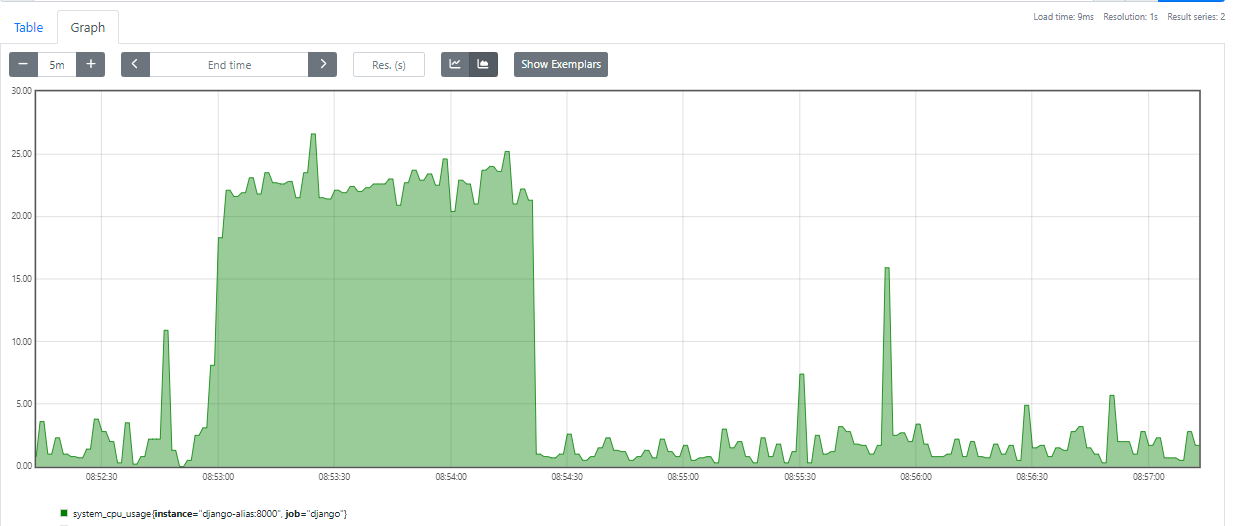
\includegraphics[width=1\textwidth]{includes/figures/tooling/performance.png}
    \caption[\ac{CPU} Auslastung der Django API]{Der erste große Anstieg zeigt die Auslastung während des Trainings eines GAN Modells (Zwischen 08:53 und 08:54), der kurze Anstieg während 08:56 zeigt die CPU Auslastung während der SSA-Algorithmus aufgerufen wurde}
    \label{fig:cpu_usage_in_container}
\end{figure}










\subsection{Ähnlichkeit der Zeitreihen der \ac{ML} Modelle}
\label{sec:similarity_of_time_series}
Um die Ähnlichkeit der Zeitreihen zu bewerten wurden die in Sektion \ref{sec:non_statistical_measures} vorgestellten Metriken genutzt.
Diese Metriken zeigen direkt, dass Beispielsweise die Ähnlichkeit der \ac{ML} Modelle basierend auf Ihrer Architektur sehr unterschiedlich ist.
Rekursive Modelle wie beispielsweise das \ac{LSTM} Modell, zeigen eine sehr viel schnellere Annährung zu den realen Daten als die generativen Modelle.
Da diese aber versuchen eine Funktion zu erlernen, welche die Daten generiert anstatt Muster aus einem Fenster an vorherigen Werten zu lernen und daraus den nächsten Wert zu berechnen, ist dies wenig verwunderlich.
Interessant ist aber, dass über einen Anstieg der Iterationen die Genauigkeit der generativen Modelle zwar tendenziell besser wird, aber von Außreißern unterbrochen wird.
Um dennoch eine vernünftige Vergleichbarkeit zu erziehlen, wurden alle Algorithmen mit der gleichen Anzahl an Iterationen trainiert. Sie wurden in Intervallen von 10, 30, 50, 70, 100, 140, 210, 300, 500 getestet. Die nativen Keras Modelle wurden noch in Intervallen von 700, 1400 und 2100 Iterationen getestet.
Für die tsgm Modelle war dies nur Teilweise noch möglich, da sich die Laufzeit im Extremfall des \ac{TGAN}s schon auf über 1h16min für 500 Iterationen belief. Da hier auch die Trainingszeit je Iteration Anstieg hätte dies, gerade über mehrere Trainingsdatensätze, zu lange gedauert und wäre daher wenig sinnvoll.

Interessante Punkte sind beispielsweise die Laufzeit der Modelle, die Anzahl an Iterationen im Verhähltnis zur Wasserstein Distanz und die Anzahl an Iterationen im Verhähltnis zur Vektor Distanz. Andere interessante Punkte sind beispielsweise das Privatsphäre Maß auch in ein Verhähltnis zur Distanz und zur Laufzeit zu setzten.
Gerade der letzte Punkt sollte interessante Ergebnisse liefern, da die generativen Modelle eine sehr hohe Laufzeit haben und daher auch ein hohes Maß an Privatsphäre bieten sollten, aber die Distanz zum original nicht zu gering sein soll, da es sonst diese nicht gut genug nachbildet.

\subsubsection{Analyse der rekursiven Modelle}
\paragraph{\textbf{RNN}}
Betrachtet man die Grafik des RNN, zeigt sich eine erhebliche Fluktuation, aber im Vergleich zu anderen Modellen weist es einen sehr stabilen Wert auf. Die Wasserstein-Distanz divergiert bei 500 Iterationen,
erreicht aber hier nur einen Wert von 0,124 – eine sehr gute Annäherung. Ähnlich verhält es sich mit der Vektordistanz, die bei nur 0,02 liegt. Beide Werte, auch die sehr niedrige Standardabweichung,
deuten auf eine hohe Übereinstimmung mit den Originaldaten hin, und das fast unmittelbar. Eine recht niedrige \ac{MIA}-Metrik zeigt ebenfalls, dass das Modell die Privatsphäre nicht ausreichend schützt und Rückschlüsse auf Originalmuster zulässt.


\paragraph{\textbf{LSTM}}
Die Daten dieses Modells verhalten sich interessant. Die Wasserstein-Distanz steigt kontinuierlich an, zeigt also eine Entfernung von den Originaldaten, allerdings in einem, verglichen mit anderen Modellen,
langsamen und geringen Rahmen. Die Standardabweichung steigt ähnlich zur Wasserstein-Distanz; gleiches gilt für die \ac{MIA}-Metrik, die leider dennoch sehr gering ist. Die Vektordistanz liegt fast bei 0 und zeigt einen Ausreißer,
der sich schnell wieder einpendelt. Aus den Daten des Mann-Whitney-U-Tests lässt sich ein Trainingseffekt erkennen, aber die P-Werte fallen nie unter die 0,05-Marke.


\begin{figure}[ht]
    \centering
    \begin{minipage}{0.5\textwidth}
        \centering
        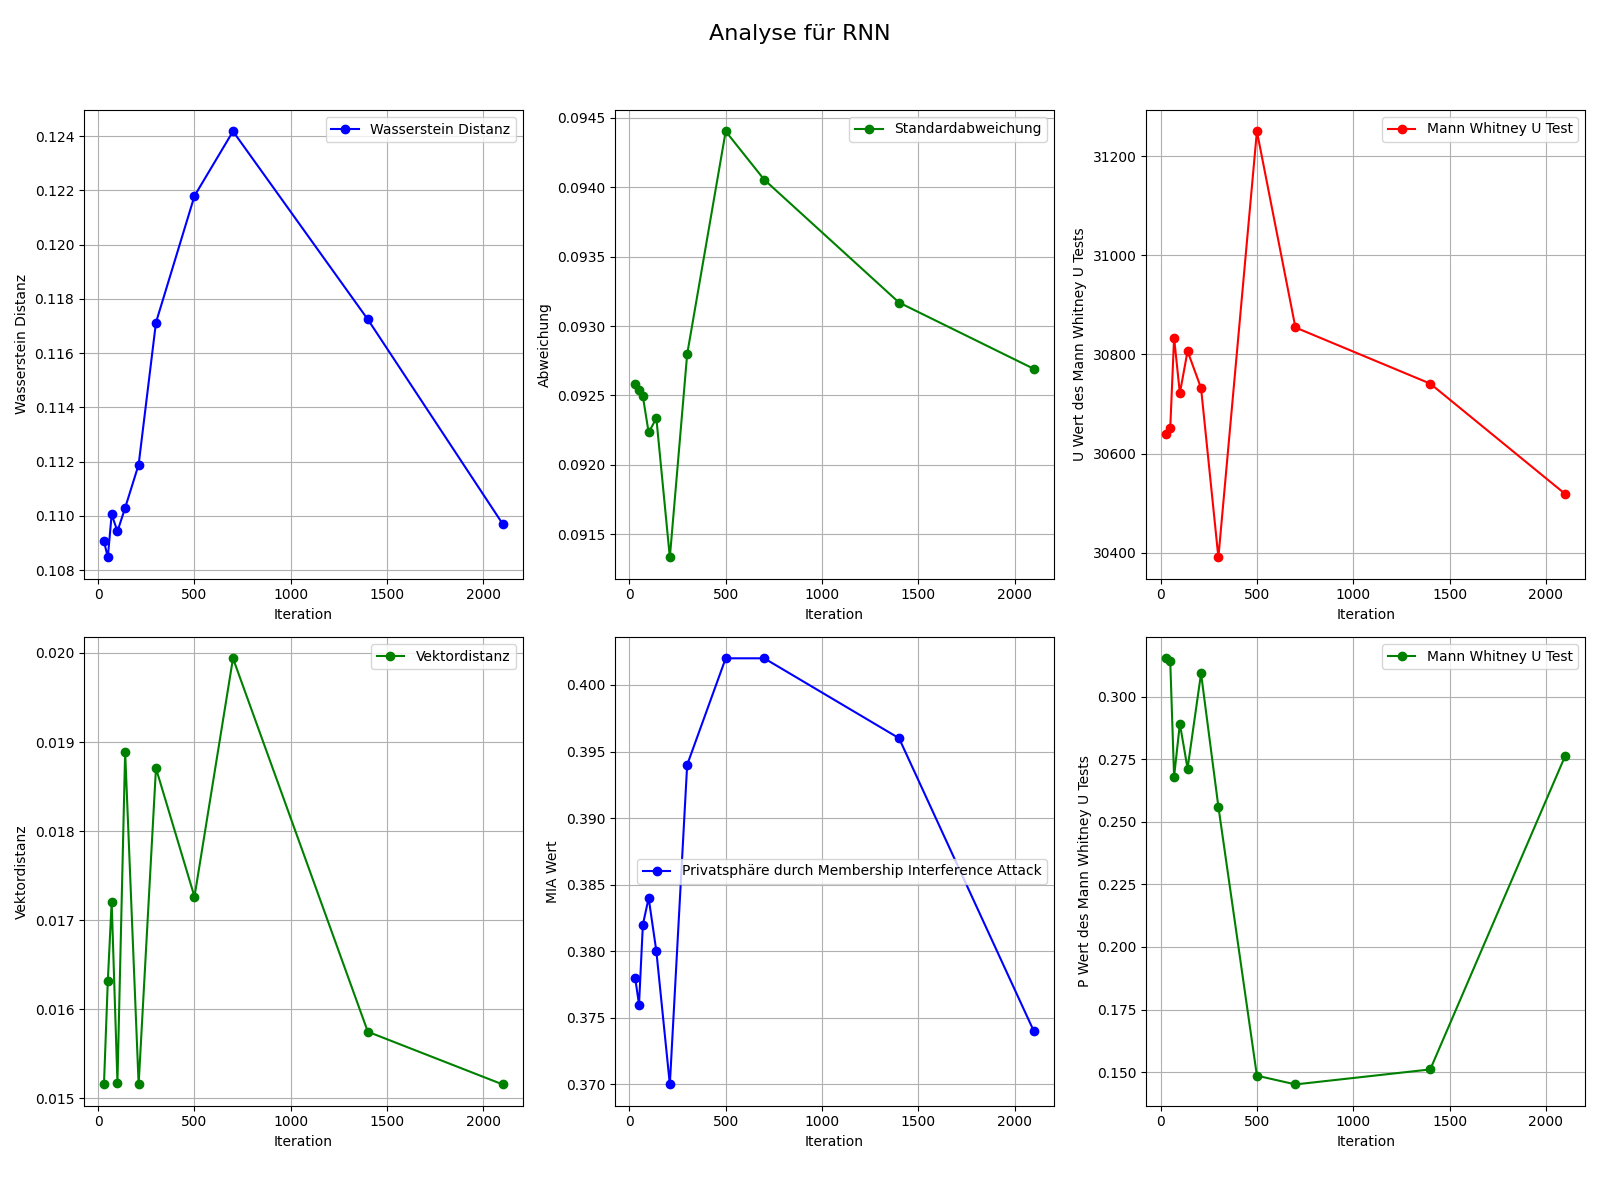
\includegraphics[width=\textwidth]{includes/figures/graphs/RNN_analysis.png}
        \caption{Analyse des RNN Modells}
        \label{fig:graphs_rnn_analysis}
    \end{minipage}\hfill
    \begin{minipage}{0.5\textwidth}
        \centering
        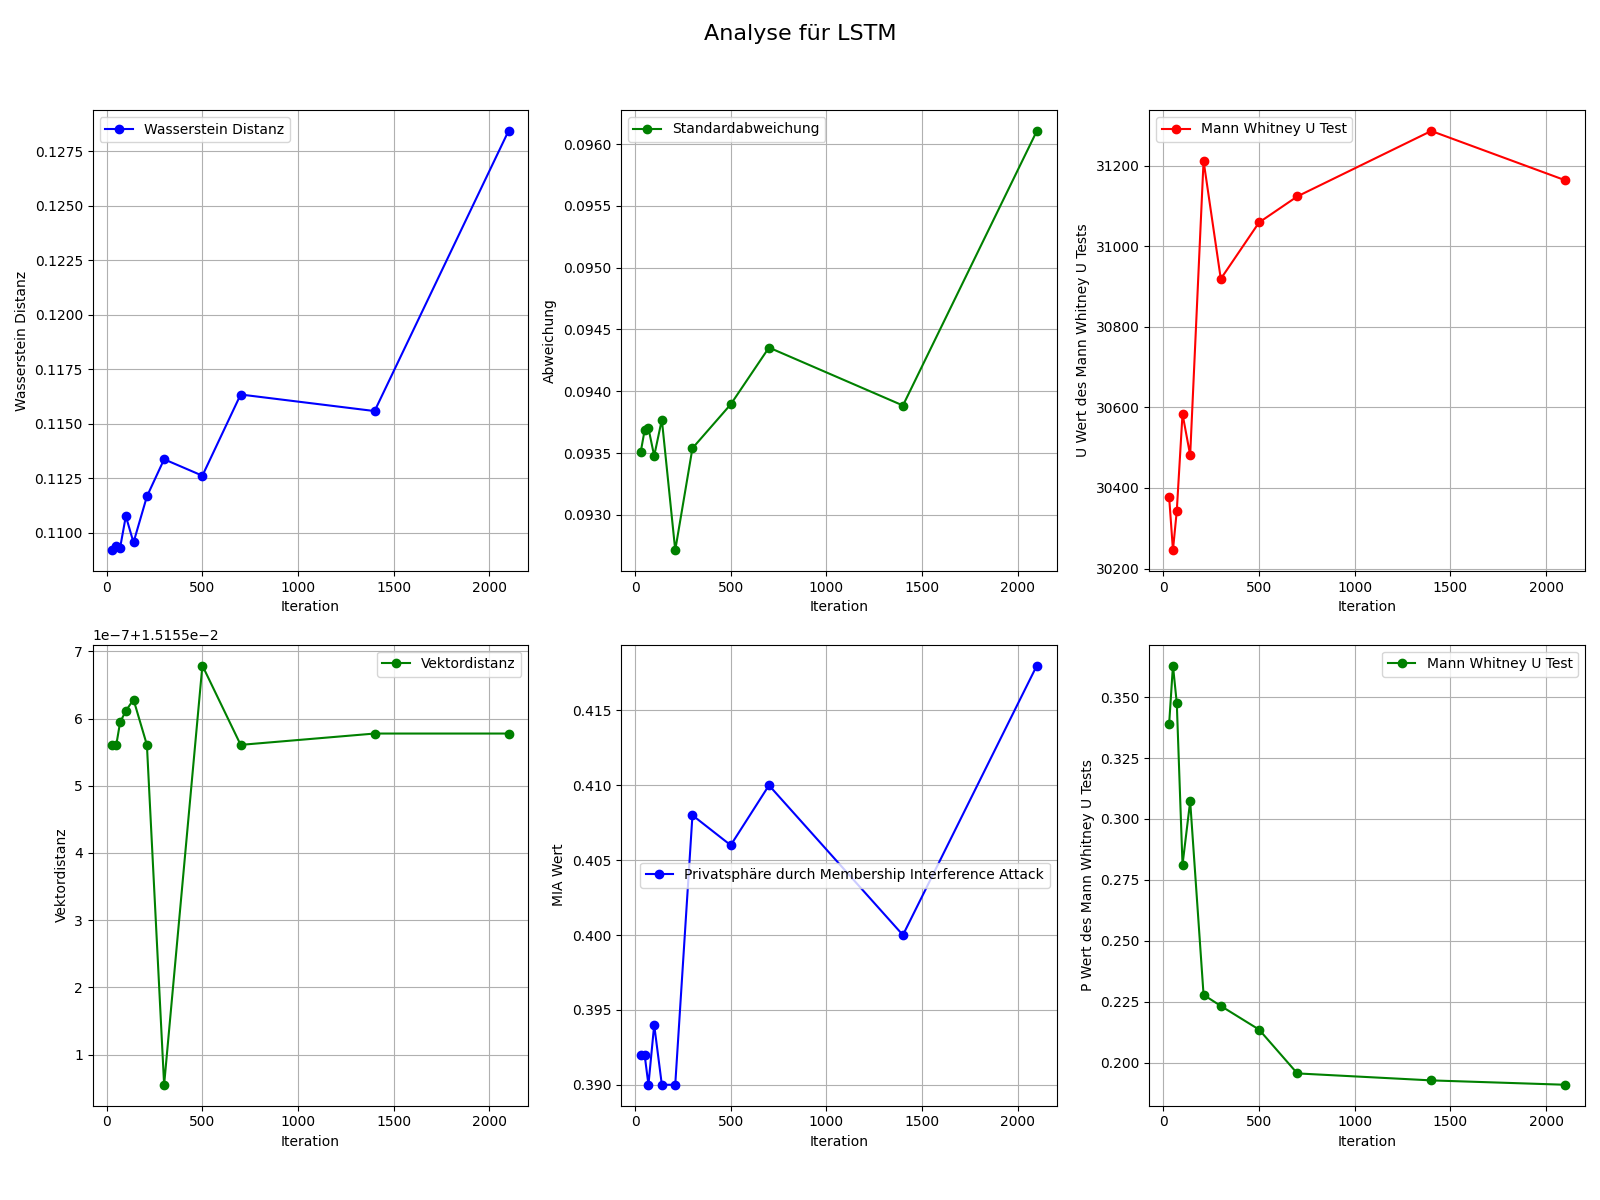
\includegraphics[width=\textwidth]{includes/figures/graphs/LSTM_analysis.png}
        \caption{Analyse des LSTM Modells}
        \label{fig:graphs_lstm_analysis}
    \end{minipage}
\end{figure}




\paragraph{\textbf{Convolutional LSTM}}
Die Wasserstein-Distanz dieses Modells startet sehr hoch, fällt schnell ab und fluktuiert, bevor sie sich bei einem Wert von 0,1 einpendelt. Das Modell kann also sehr schnell die Verteilung der Originaldaten erfassen.
Ähnlich verhält es sich mit der Vektordistanz, die ebenfalls hoch beginnt und sich etwas langsamer einpendelt als die Wasserstein-Distanz. Mit einem Wert von ungefähr 0,45 ist sie aber dennoch akzeptabel.
Die \ac{MIA}-Metrik und die Standardabweichungen folgen einem ähnlichen Verlauf: Sie starten hoch, fallen, fluktuieren und pendeln sich ein. Am Ende erreicht das Modell nur einen Wert von 0,65 in der \ac{MIA},
was recht gut ist. Die Ergebnisse des Mann-Whitney-U-Tests zeigen niedrige P-Werte, die aber nie den Schwellwert von 0,05 erreichen. Das Modell erreicht somit nie eine exakte Annäherung an die Originaldaten,
was durchaus erwünscht sein kann. Der starke Anstieg um Iteration 1400 sollte durch weitere Tests untersucht werden.

\paragraph{\textbf{CNN LSTM}}
Die Wasserstein-Distanz zeigt bei ungefähr 700 Iterationen eine signifikante Spitze. Da der Wert über mehrere Datensätze hinweg berechnet wurde und die Extrema nicht stärker als bei anderen Iterationen abweichen,
scheint das Modell in diesem Bereich zu divergieren. Die Standardabweichung zeigt keine Auffälligkeiten. Die Vektordistanz verhält sich ähnlich wie die Wasserstein-Distanz, nur mit einem niedrigeren Wert, der gegen Ende
der Iterationen wieder ansteigt. Interessant ist der Abfall der \ac{MIA}-Metrik, als die Wasserstein- und Vektordistanz ansteigen, was etwas kontraintuitiv erscheint. Die Werte des Mann-Whitney-U-Tests zeigen ähnliche Muster
und normalisieren sich nach der initialen Trainingsphase.

\begin{figure}[ht]
    \centering
    \begin{minipage}{0.5\textwidth}
        \centering
        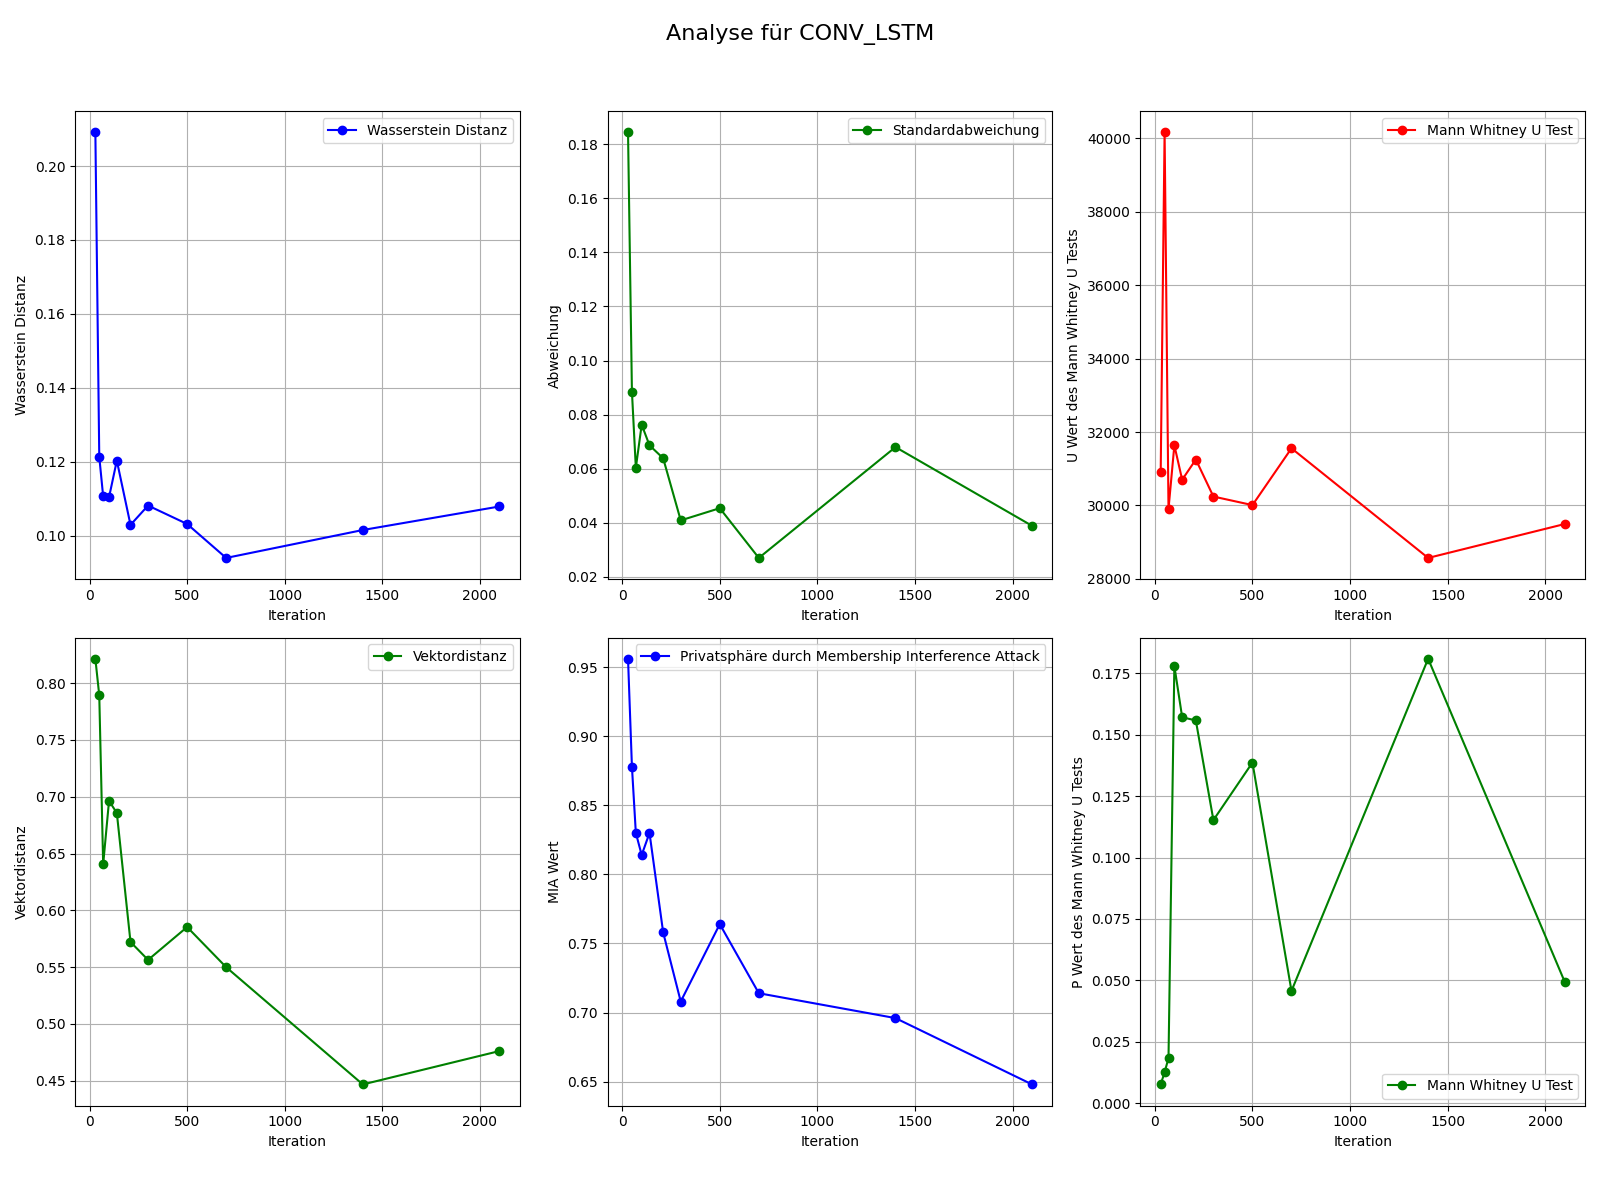
\includegraphics[width=\textwidth]{includes/figures/graphs/CONV_LSTM_analysis.png}
        \caption{Analyse des Convolutional LSTM Modells}
        \label{fig:graphs_conv_analysis}
    \end{minipage}\hfill
    \begin{minipage}{0.5\textwidth}
        \centering
        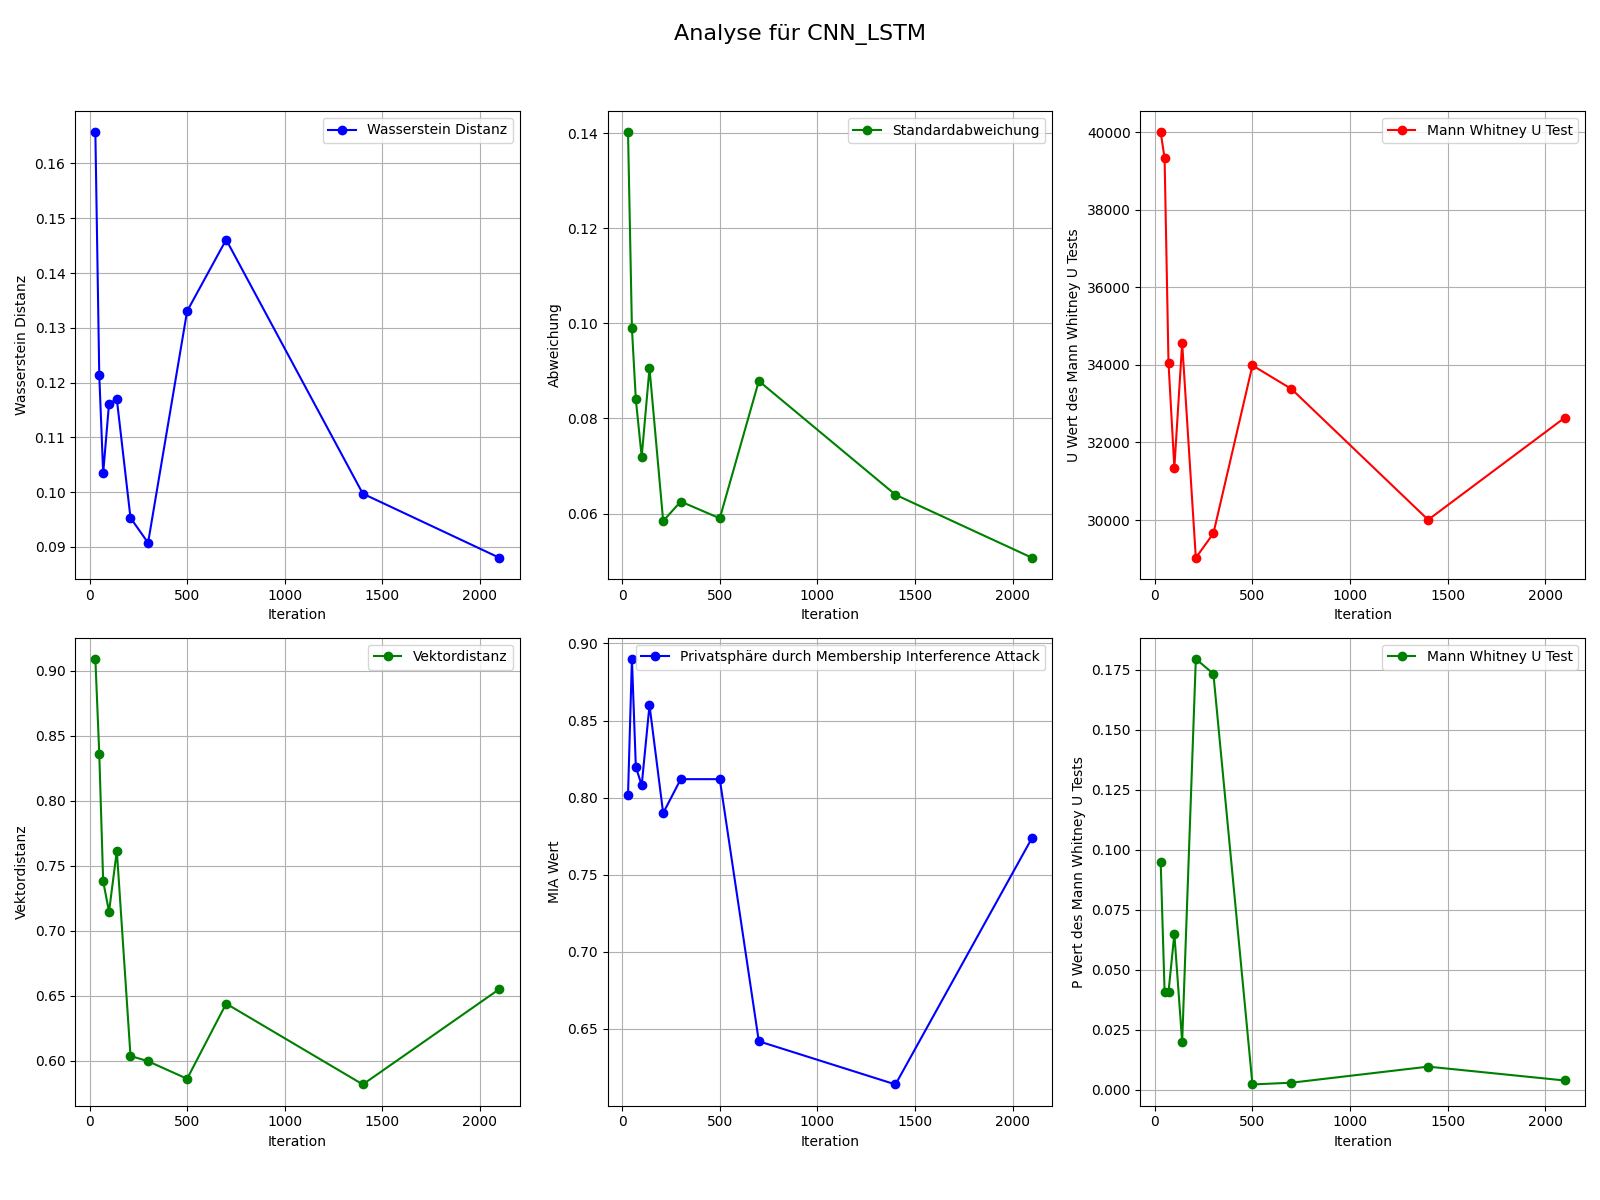
\includegraphics[width=\textwidth]{includes/figures/graphs/CNN_LSTM_analysis.png}
        \caption{Analyse des CNN LSMT Modells}
        \label{fig:graphs_cnn_analysis}
    \end{minipage}
\end{figure}



\subsubsection{Analyse der generativen Modelle}

\paragraph{\textbf{GAN}}
Das GAN zeigte eine signifikante anfängliche Verbesserung und verringerte schnell die Diskrepanz in der Verteilung zwischen generierten und realen Daten, wie die Wasserstein- und Vektordistanz-Metriken anzeigen.
Die Standardabweichung des Modells nimmt ab, was auf eine Verbesserung der Konsistenz der Datengenerierung hindeutet.

Schwankungen in der Mann-Whitney-U-Test-Statistik und ihren P-Werten weisen auf Momente der Divergenz zwischen den synthetischen und realen Datenverteilungen hin, was auf eine potenzielle Überanpassung oder
Instabilität des Modells im Laufe des Trainings schließen lässt. Die \ac{MIA}-Werte deuten auf eine erhöhte Anfälligkeit für Inferenzangriffe hin, sind aber verglichen mit anderen Algorithmen recht gut.

Die anfänglichen und schnellen Erfolge des Modells zeigen einen schnellen Lernprozess, der ab ungefähr 1000 Iterationen stagniert.


\paragraph{\textbf{TGAN}}
Das TGAN zeigte gute Fähigkeiten bei der Annäherung an reale Datenverteilungen, wie die Trends der Wasserstein- und Vektordistanz zeigen. Bereits die ersten Iterationen des Modells zeigen Fortschritte bei der
Generierung von synthetischen Daten. Gleichzeitig zeigte das TGAN Schwankungen in den Datenschutzmetriken, was eine Konsequenz der schnellen Verbesserung der Wasserstein- und Vektordistanzmetriken sein kann.

Die beobachtete Standardabweichung und die Mann-Whitney-U-Test-Statistiken wiesen zudem auf Perioden signifikanter Verbesserung und Stabilität in der Leistung des TGAN hin. Diese Metriken wiesen jedoch auch auf
Fälle hin, in denen die Ergebnisse des Modells von den gewünschten Ergebnissen abwichen, was auf potenzielle Bereiche zur Verfeinerung hindeutet.


\begin{figure}[ht]
    \centering
    \begin{minipage}{0.5\textwidth}
        \centering
        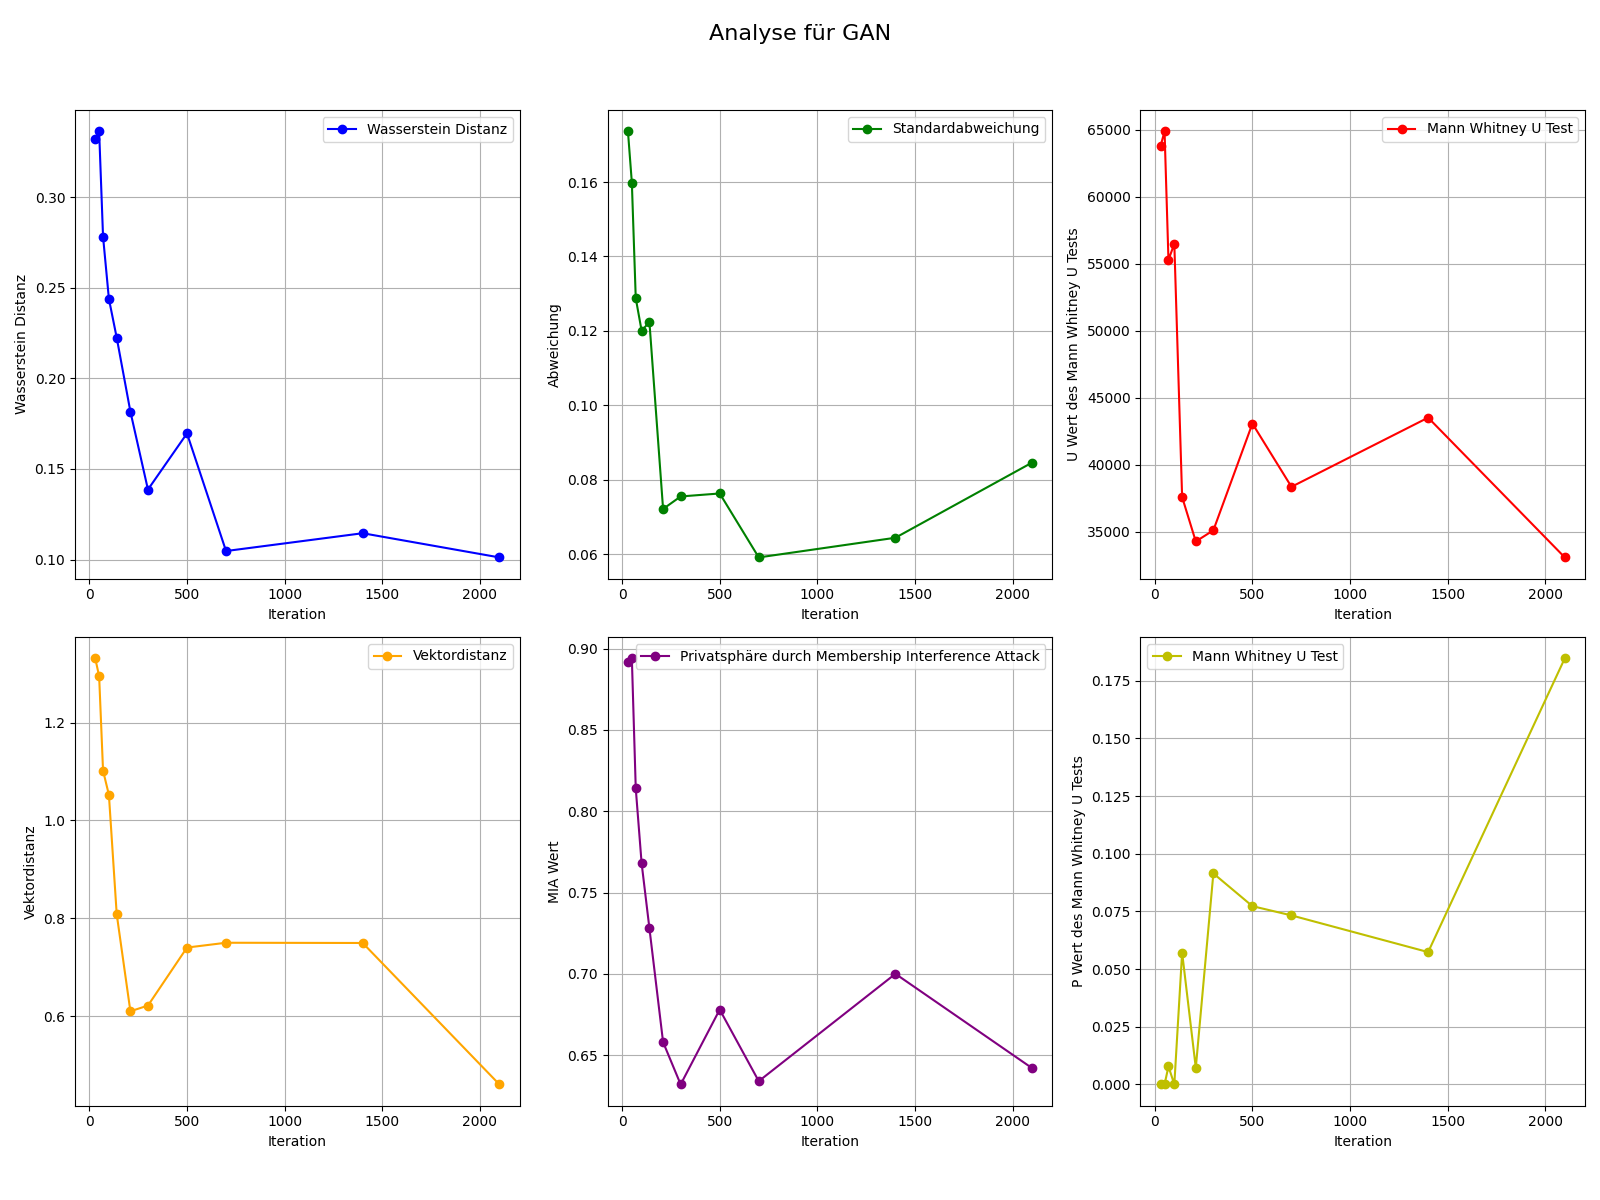
\includegraphics[width=\textwidth]{includes/figures/graphs/GAN_analysis.png}
        \caption{Analyse des GAN Modells}
        \label{fig:graphs_gan_analysis}
    \end{minipage}\hfill
    \begin{minipage}{0.5\textwidth}
        \centering
        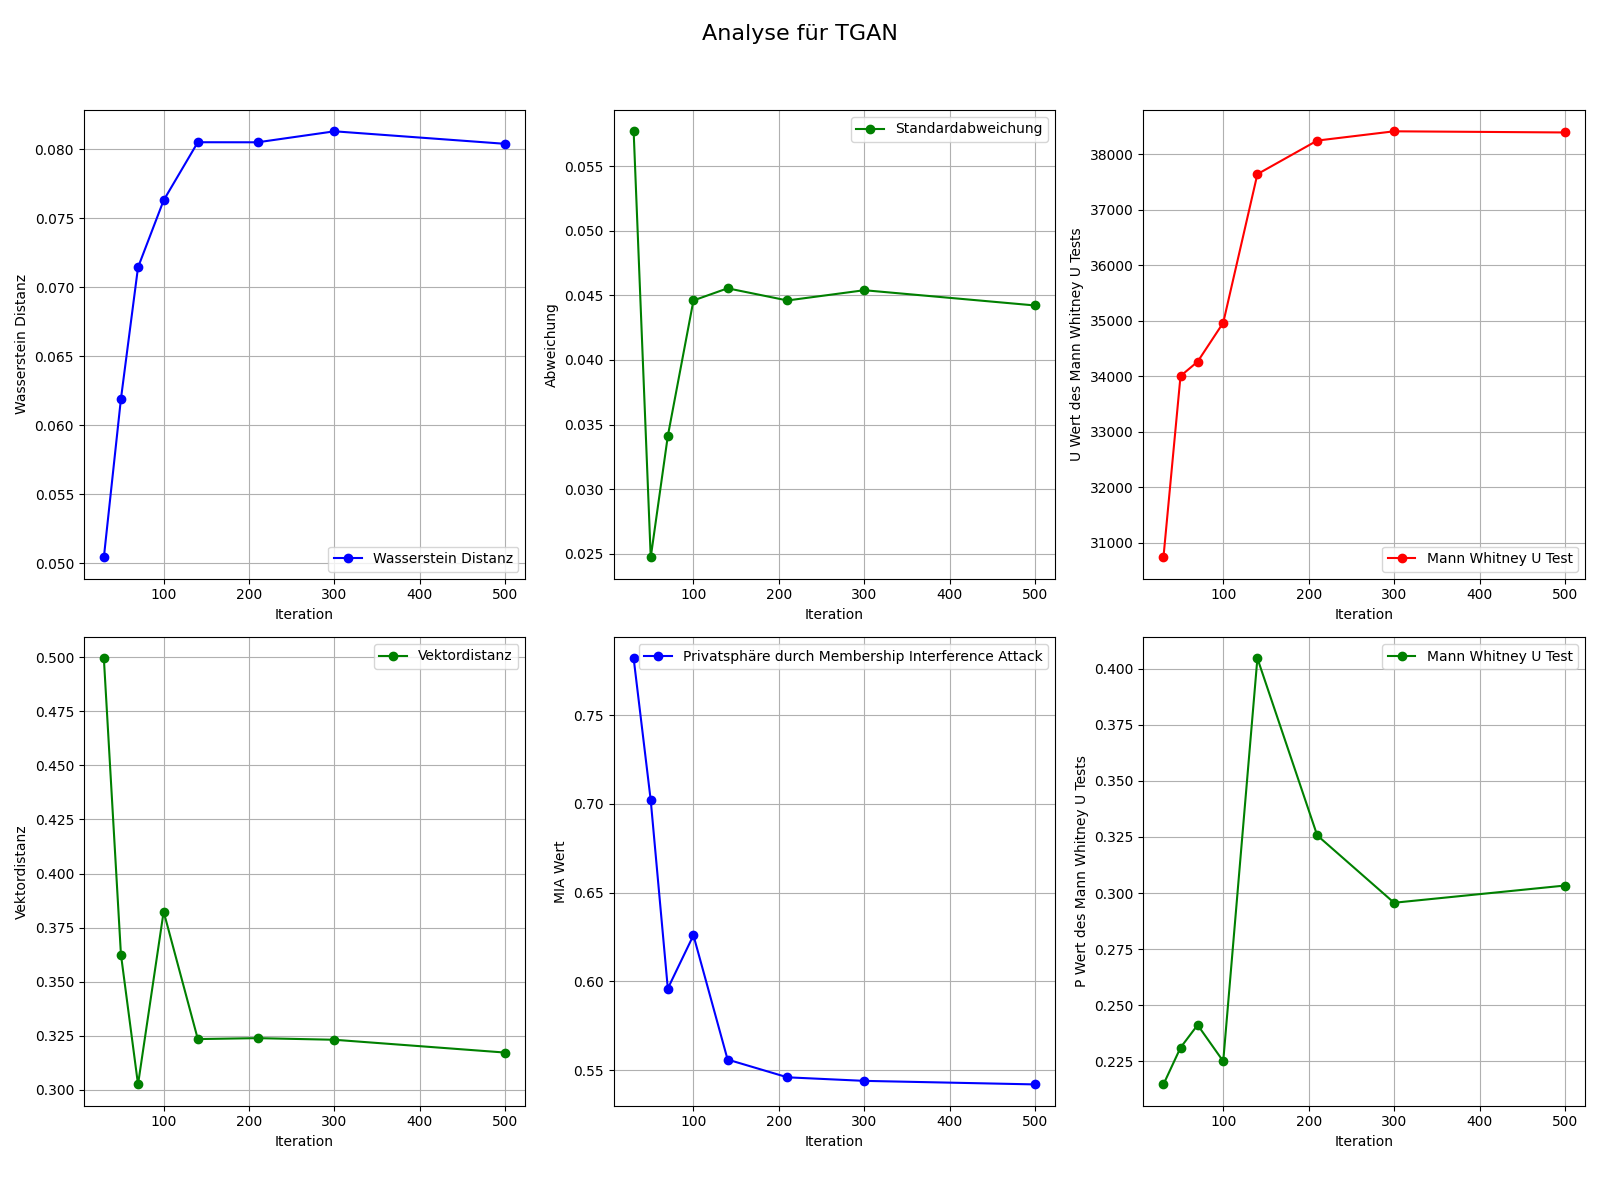
\includegraphics[width=\textwidth]{includes/figures/graphs/TGAN_analysis.png}
        \caption{Analyse des TGAN Modells}
        \label{fig:graphs_tgan_analysis}
    \end{minipage}
\end{figure}


\paragraph{\textbf{TCGAN}}
Während des gesamten Trainingsprozesses zeigte das TCGAN eine gute Verbesserung mit einem abfallenden Lerneffekt, wie die Werte der Standardabweichung, Vektordistanz und Wasserstein-Distanz anzeigen.

Bezüglich der Privatsphäre zeigte das TCGAN eine schlechte Leistung, wie die \ac{MIA}-Metrik zeigt.

Darüber hinaus wiesen die P-Werte des Mann-Whitney-U-Tests auf Momente hin, in denen sich die synthetischen Daten signifikant von den Originaldaten unterschieden, was Fragen hinsichtlich der Fähigkeit des Modells aufwirft,
Daten mit konsistenten statistischen Eigenschaften über Iterationen hinweg zu generieren.
\begin{figure}[ht]
    \centering
    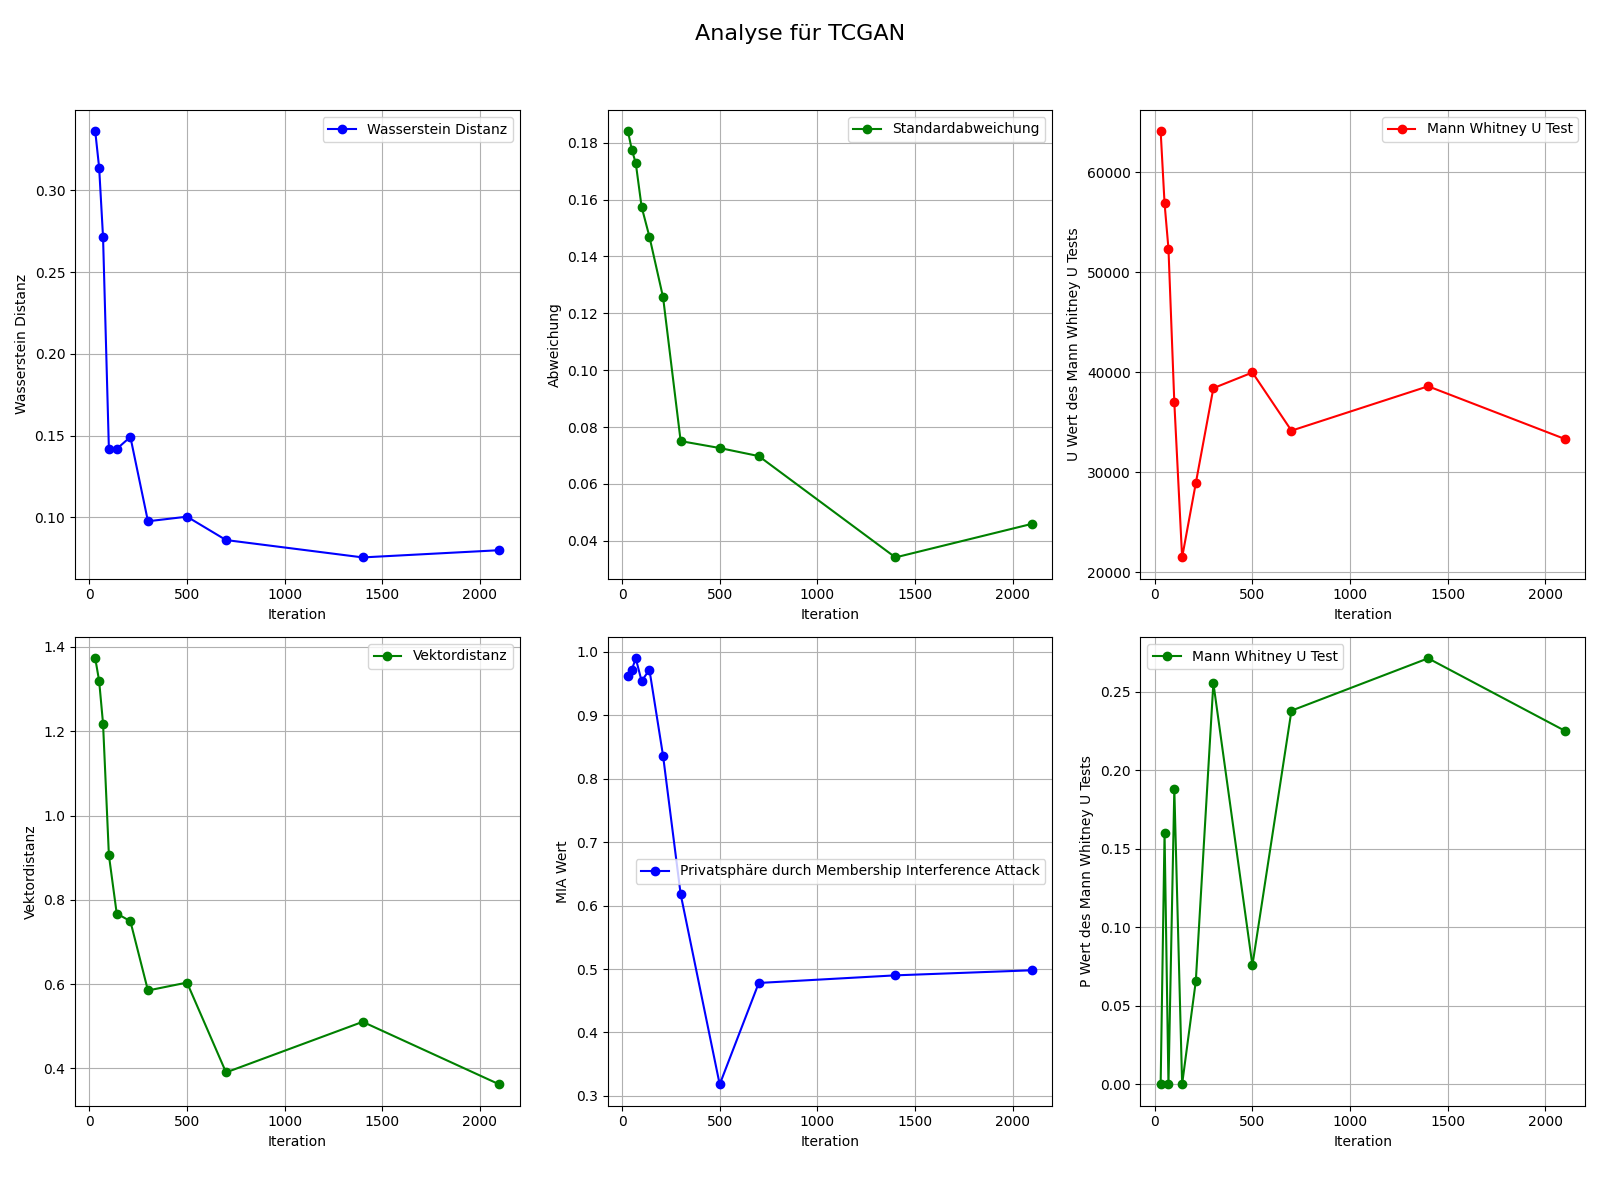
\includegraphics[width=1\textwidth]{includes/figures/graphs/TCGAN_analysis.png}
    \caption{Analyse des TCGAN Modells}
    \label{fig:graphs_tcgan_analysis}
\end{figure}


\paragraph{\textbf{CGAN-keras}}
Die CGAN-Keras zeigten einen sehr guten Start mit einer steilen Verbesserung des Wasserstein-Abstands und einem erstaunlich niedrigen Ausgangswert. Die Vektordistanz zeigt einen ähnlichen Verlauf, nähert sich extrem schnell den Daten an und
entfernt sich dann wieder. Hier ist eine hohe Fluktuation zu beobachten. Trotzdem sind die Standardabweichungen sehr gering und die Privatsphäre-Metriken zeigen einen durchaus guten Wert mit einer steigenden Tendenz.
Die Analyse der Mann-Whitney-U-Test-Statistiken und der P-Werte ergab jedoch Zeiträume, in denen die statistischen Eigenschaften der synthetischen Daten signifikant von denen der realen Daten abwichen, während zu manchen Zeiten der Schwellwert von 0,05 unterschritten wurde.

\paragraph{\textbf{CGAN-tsgm}}
Die CGAN-Variante der tsgm-Bibliothek zeigt ähnlich gute und schnelle Annäherungen und Trainingsfortschritte wie die keras-Variante. Nach einer rapiden Lernphase pendeln sich die Werte ein und zeigen eine gute Annäherung an die Originaldaten,
wie sich anhand der Wasserstein- und Vektordistanz sowie der Standardabweichung ablesen lässt. Leider zieht das gute Erlernen auch Konsequenzen für die Privatsphäre nach sich, da die \ac{MIA}-Metrik einen sehr niedrigen Wert zeigt.


\begin{figure}[ht]
    \centering
    \begin{minipage}{0.5\textwidth}
        \centering
        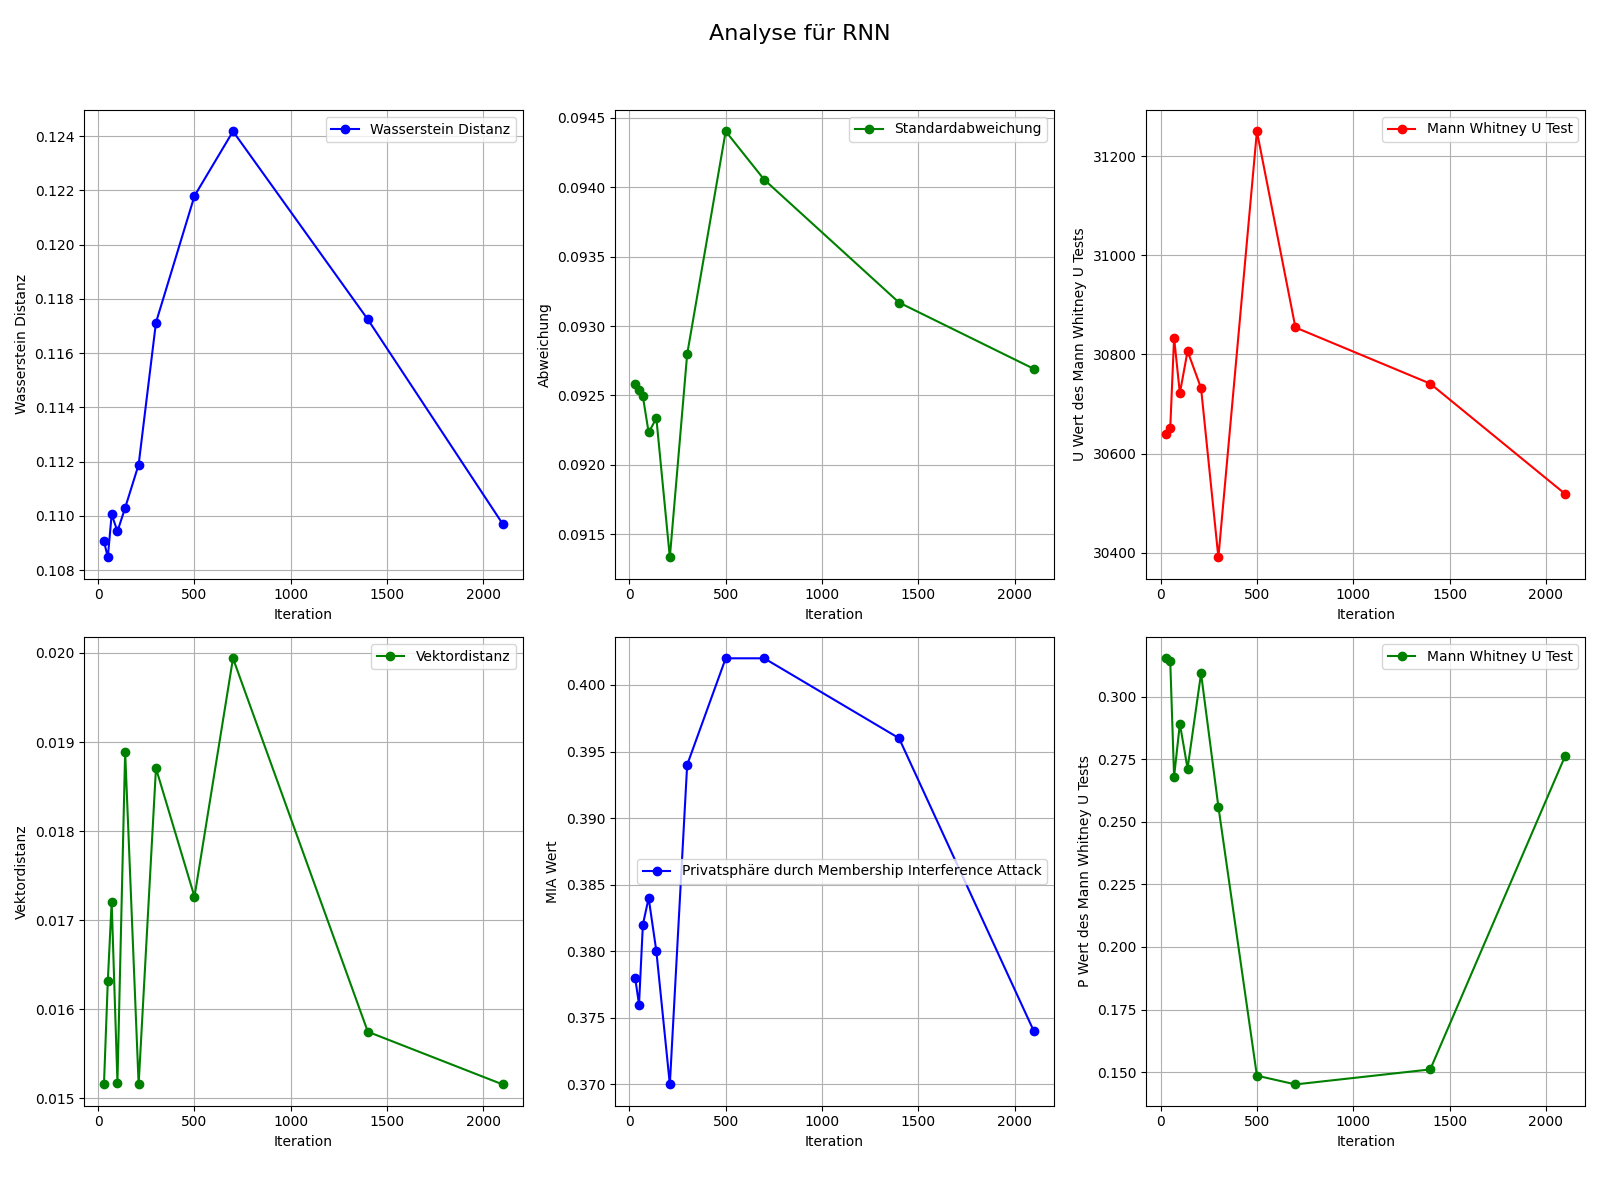
\includegraphics[width=\textwidth]{includes/figures/graphs/RNN_analysis.png}
        \caption{Analyse des CGAN tsgm Modells}
        \label{fig:graphs_cgan_tsgm_analysis}
    \end{minipage}\hfill
    \begin{minipage}{0.5\textwidth}
        \centering
        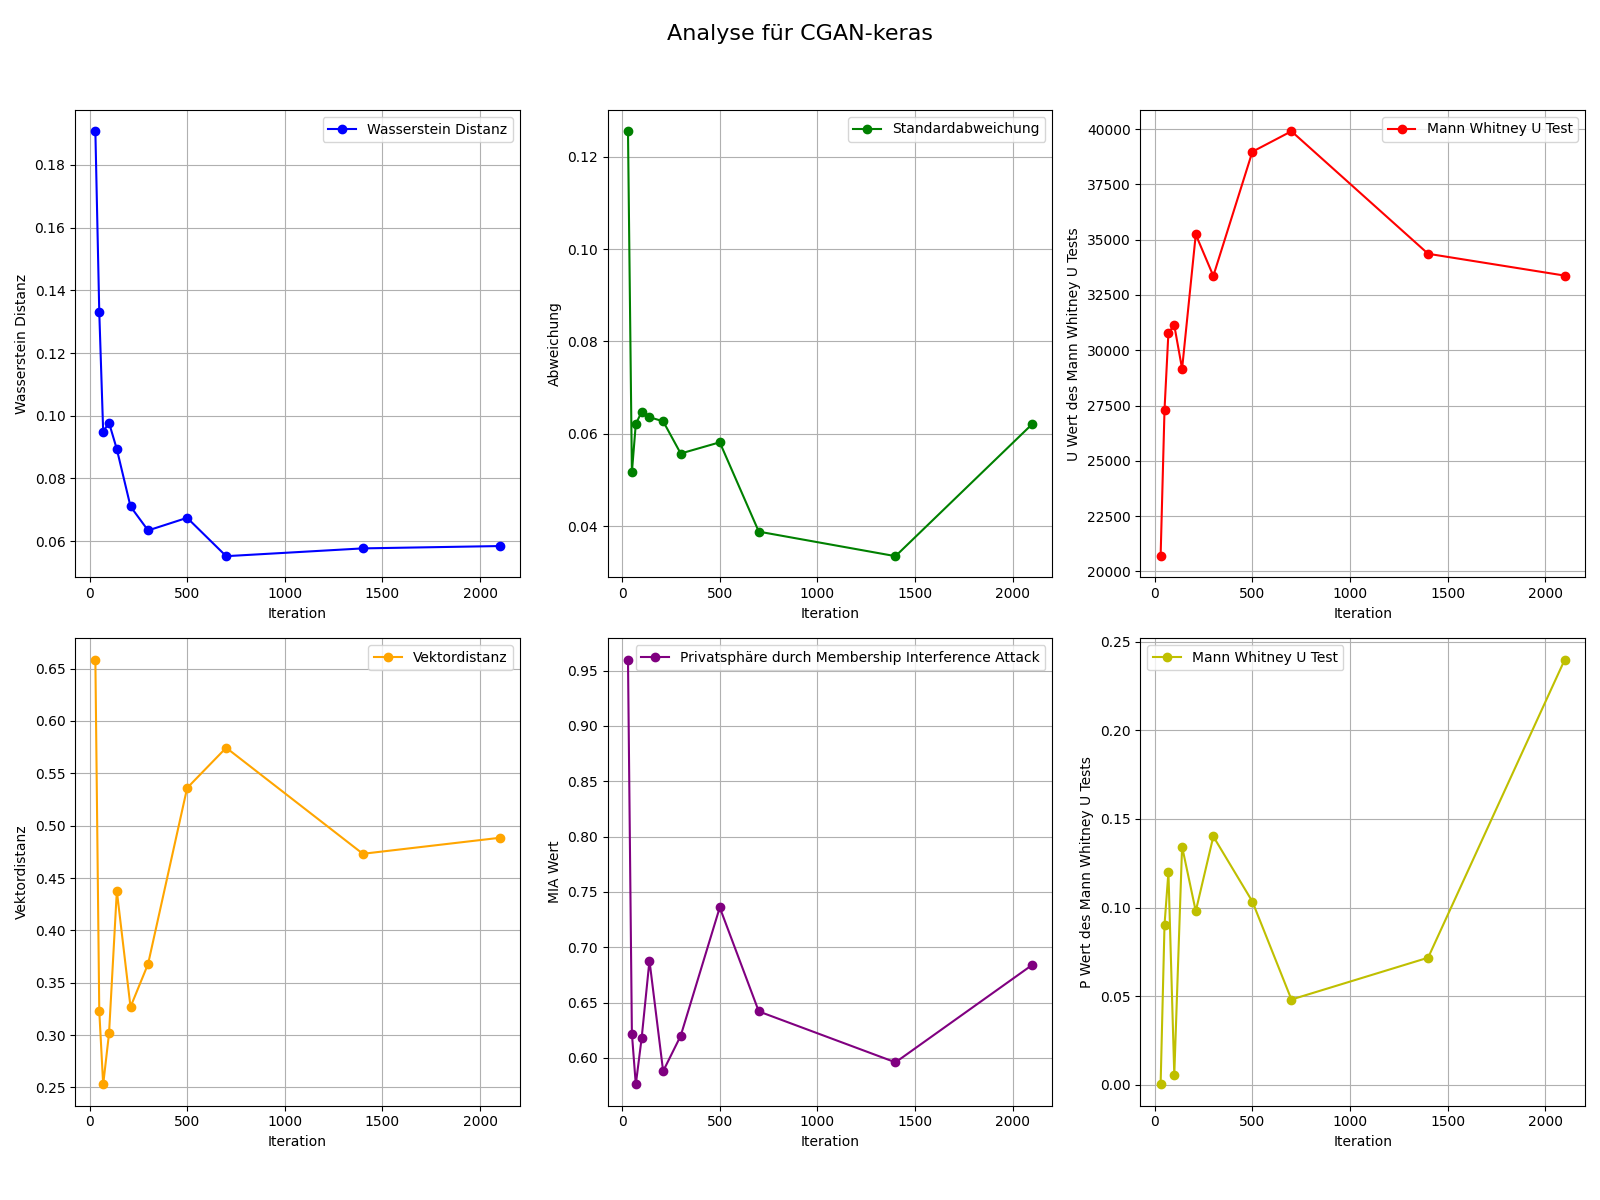
\includegraphics[width=\textwidth]{includes/figures/graphs/CGAN-keras_analysis.png}
        \caption{Analyse des CGAN Keras Modells}
        \label{fig:graphs_cgan_keras_analysis}
    \end{minipage}
\end{figure}




Da in den vorherigen Abschnitten primär die reinen Verteilungen über verschiedene Datensätze gezeigt wurden, ist es auch interessant zu sehen, wie sich die einzelnen Modelle auf die einzelne Datensätze auswirken.
Da die Modelle (mit ausnahme der tsgm Modelle) in der Lage sind spezifisch für die einzelnen Datensätze passende synthetische Varianten zu generieren, lässt sich die jeweilige Iteration eine Histogramms der synthetischen Daten erstellen, in dem sowohl die Verteilung als auch die direkten Werte verglichen werden.

Wie Anhand der in Abbildung \ref{fig:sinus_histogram} und \ref{fig:sinus_histogram_compare} gezeigten Histogramme zu sehen ist, sind die synthetischen Daten sehr gut an die Originaldaten angepasst. Es gibt, auch nach etwa 2100 Iterationen noch unterschiede im CGAN-keras Modell zu sehen, diese sind aber nur minimal, da es aber auch  das Ziel war die synthetischen Daten dem original nur anzunähern, scheint dieses Ergebnis doch durchaus gut.
\begin{figure}[ht]
    \centering
    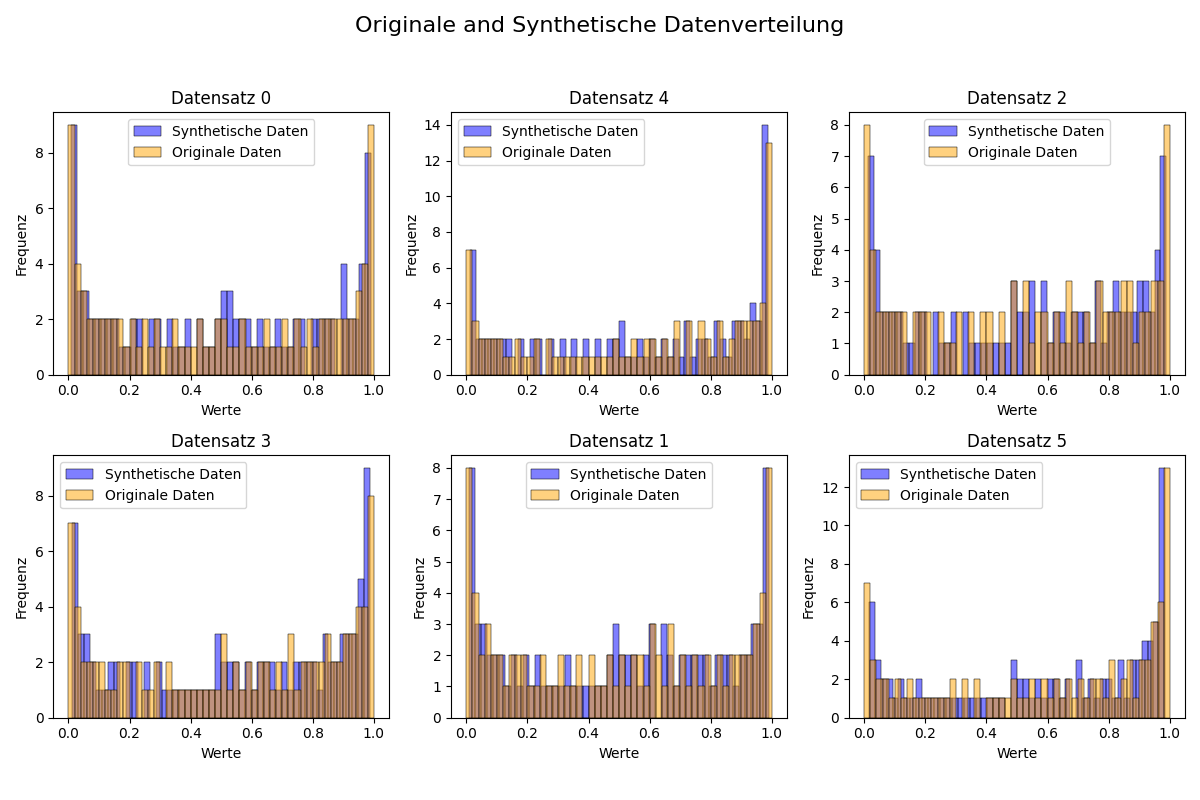
\includegraphics[width=1\textwidth]{includes/figures/graphs/sinus_plot_histogram.png}
    \caption{Verteilungen des jeweiligen einzelnen Trainingsdaten zu ihren synthetischen Varianten}
    \label{fig:sinus_histogram}
\end{figure}


\begin{figure}[ht]
    \centering
    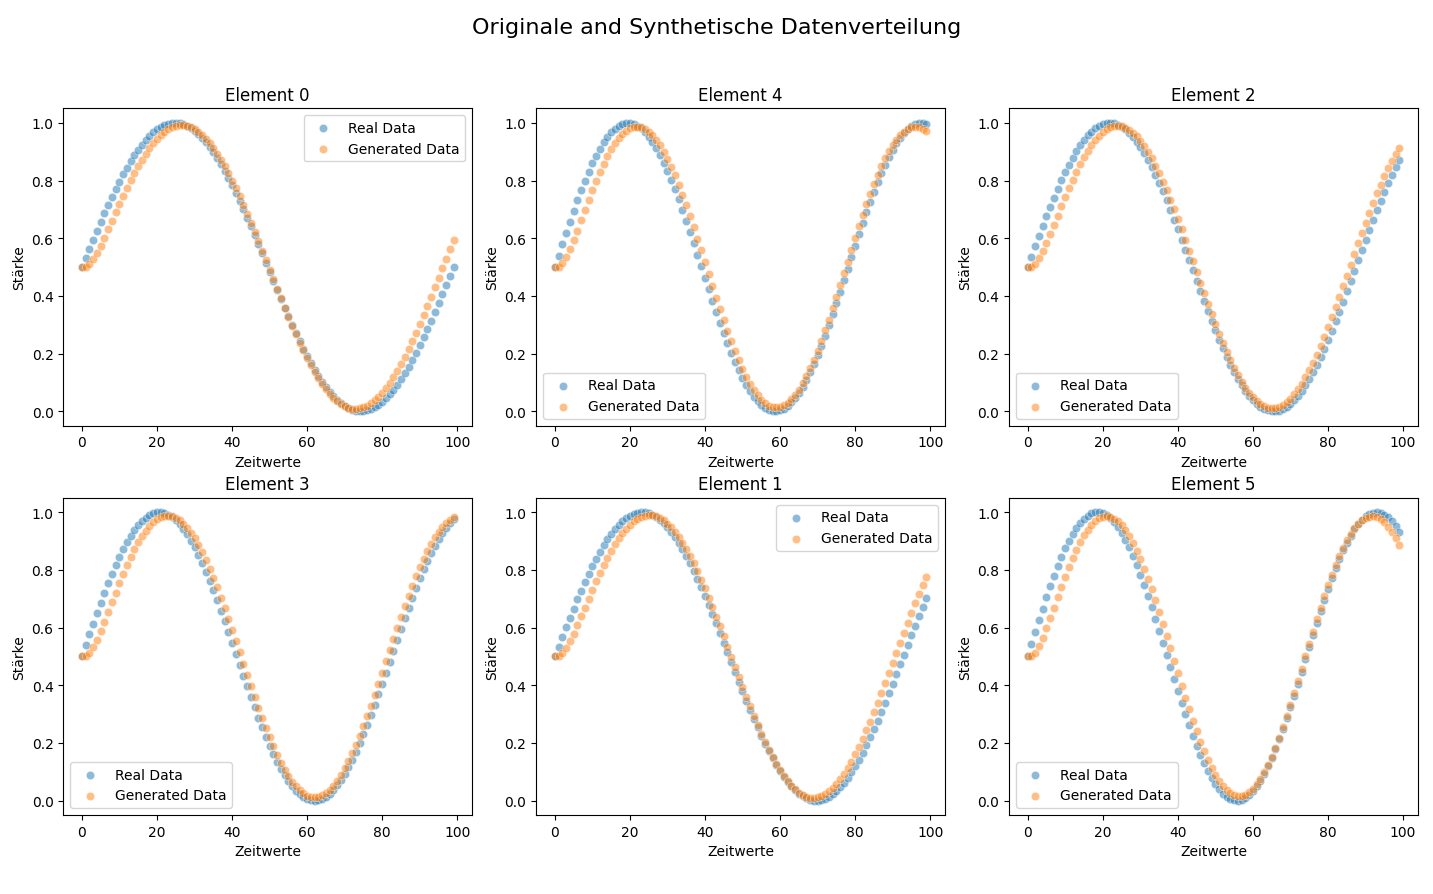
\includegraphics[width=1\textwidth]{includes/figures/graphs/sinus_plot_histgram_compare.png}
    \caption{Vergleich der einzelnen Trainingdaten zu ihren synthetischen Varianten}
    \label{fig:sinus_histogram_compare}
\end{figure}


\subsection{Ähnlichkeit der Zeitreihen der TSA Modelle}
\label{sec:similarity_of_time_series_tsa}
Um einen Vergleich von den \ac{TSA} Algorithmen zu den \ac{ML} Modellen zu ermöglichen, wurden gerade beim \ac{SSA} und \ac{EMD} Algorithmus ein paar Veränderungen vorgenommen.
Da diese ja mit \ac{IMF}s arbeiten, kann die Genauigkeit der Rückgabe über die verschiedenen \ac{IMF}s variieren. Daher wurden die Tests mit steigender Anzahl an \ac{IMF}s durchgeführt.
Bei Modellen wie AMIRA oder Cubic-Spline war dies nicht ganz möglich, weshalb hier die Metriken nicht variieren und sich nur auf das Gesammtergebnis beziehen.


\subsubsection{Analyse von \ac{SSA} und \ac{EMD}}


\begin{figure}[ht]
    \centering
    \begin{minipage}{0.5\textwidth}
        \centering
        \includegraphics[width=\textwidth]{includes/figures/graphs/emd_analysis.png}
        \caption{Analyse des EMD Algorihtmus}
        \label{fig:graphs_emd_analysis}
    \end{minipage}\hfill
    \begin{minipage}{0.5\textwidth}
        \centering
        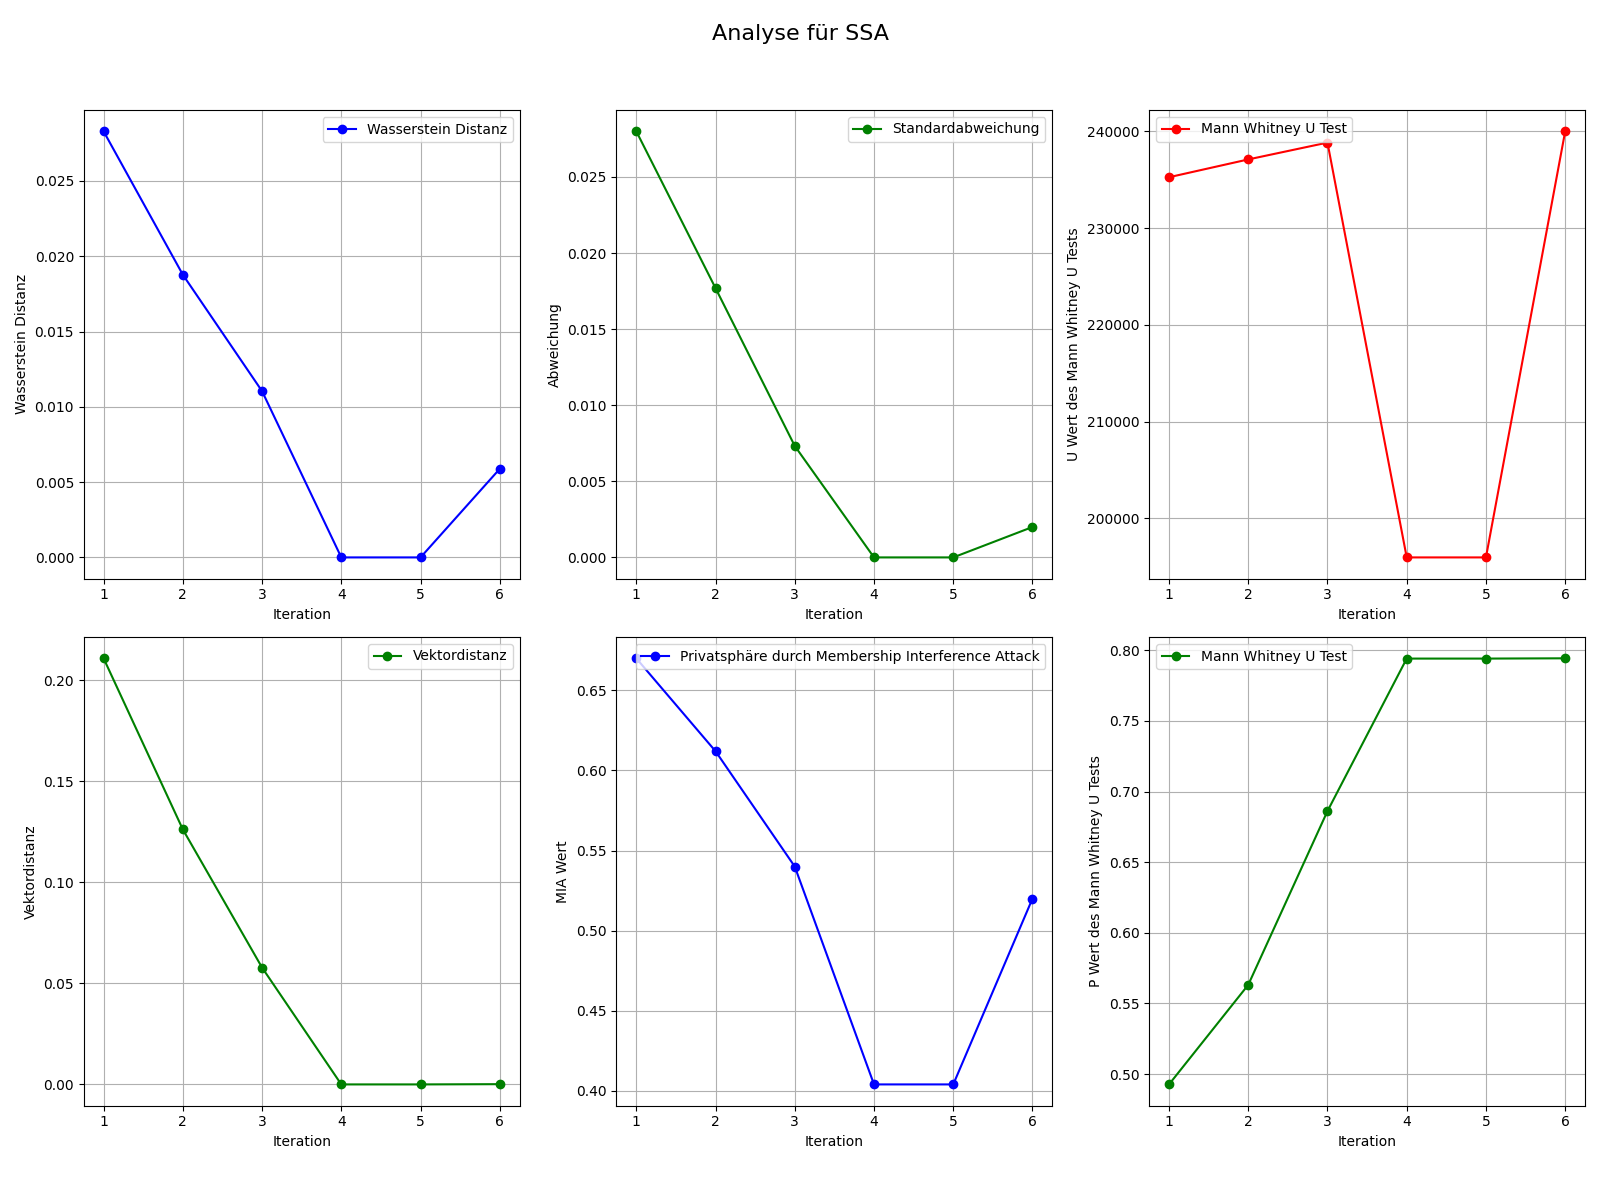
\includegraphics[width=\textwidth]{includes/figures/graphs/SSA_analysis.png}
        \caption{Analyse des SSA Algorihtmus}
        \label{fig:graphs_ssa_analysis}
    \end{minipage}
\end{figure}

\paragraph{\textbf{SSA}}
Der SSA Algorithmus zeigt, wie zu erwarten ist einen enormen Abfall in der Wasserstein Distanz sowie der Vektor Distanz und der Standardabweichung. Dies ist soweit auch verständlich, da hier mehr Informationen aus dem originalen Signal übernommen werden.
Aber der Anstieg am Ende, in der alle \ac{IMF}s genutzt werden ist interessant. Da die \ac{IMF}s aber mit steigender Position die entsprechend Elemente der Reihe aufnehmen, könnte dies im Vergleich zur gesammten analysierten Datenmenge eine Entfernung von der originalen Verteilung mitsich ziehen. Die Vektordistanz ist davon ja nicht betroffen.
Spannend ist die \ac{MIA} Metrik, da diese einen erstaunlichen hohen Wert zeigt, und dies obwohl die Vektordistanz sehr niedrig ist, also eine gute Angleichung andeutet. Schaut man auf die Ergebnisse des Mann Whitney U Tests, so steigen diese an, anstatt abzufallen. Während dies eigentlich eine Entfernung von originalen Daten darstellen sollte, zeigen die anderen Metriken genau das Gegenteil.
Dies müsste genauer untersucht werden.

\paragraph{\textbf{EMD}}
Der EMD Algorithmus zeigt ein sehr ähnliches Bild zu \ac{SSA} Algorithmus und zeigt den Abfall in  Standardabweichung, Wasserstein- und Vektor Distanz mit einem Anstieg, sofern alle \ac{IMF}s einbezogen werden.
Ein gleiches Verhalten zeigt auch die \ac{MIA} Metrik, welche einen sehr hohen Wert zeigt, obwohl die anderen Metriken eine gute Angleichung andeuten.
Hier steigt aber zwischenzeitlich der P-Wert des Mann Whitney U Tests enorm an, fällt aber wieder auf einen normalen Wert und stabilisiert sich hier. Auch dies ist interessant und sollte genauer untersucht werden.


\subsubsection{Analyse von AMIRA und Cubic Spline}
Da beide Modelle nicht auf ähnliche Weise flexibel sind wie die vorherigen Modelle und Algorithmen ist es hier nicht möglich eine Unterscheidung zwischen Iterationen oder \ac{IMF}s zu treffen.
Daher lies sich nur ein Wert jeweil berechnen.
Beide Varianten besitzen einen sehr niedrigen Wert in der Wasserstein- und Vektordistanz sowie in der Standardabweichung, relativ hohe Werte in der \ac{MIA} Metrik und einen recht hohen \textit{p} Wert im Mann Whitney U Test.



\begin{figure}[ht]
    \centering
    \begin{minipage}{0.5\textwidth}
        \centering
        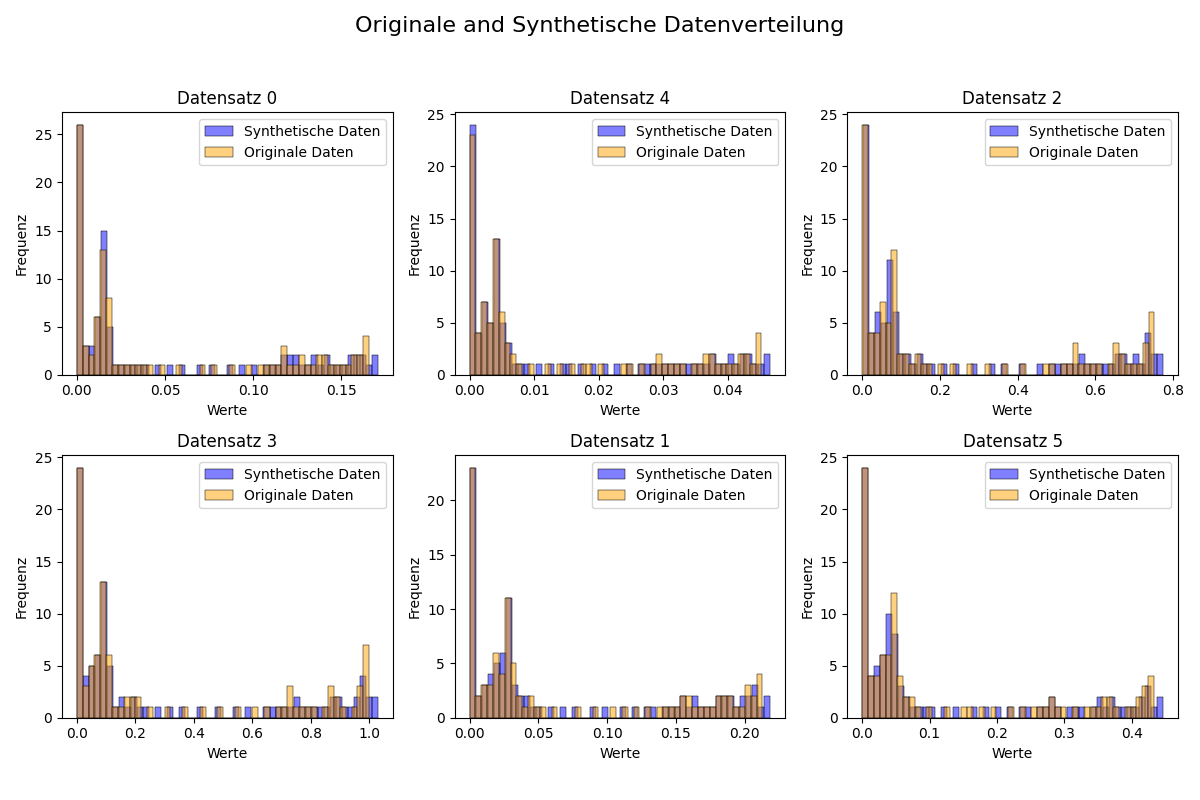
\includegraphics[width=\textwidth]{includes/figures/graphs/corona_histogram_tsa.png}
        \caption{Verteilung der originalen Daten mit den synthetischen Daten des SSA Algorihtmus}
        \label{fig:graphs_ssa_histogram}
    \end{minipage}\hfill
    \begin{minipage}{0.5\textwidth}
        \centering
        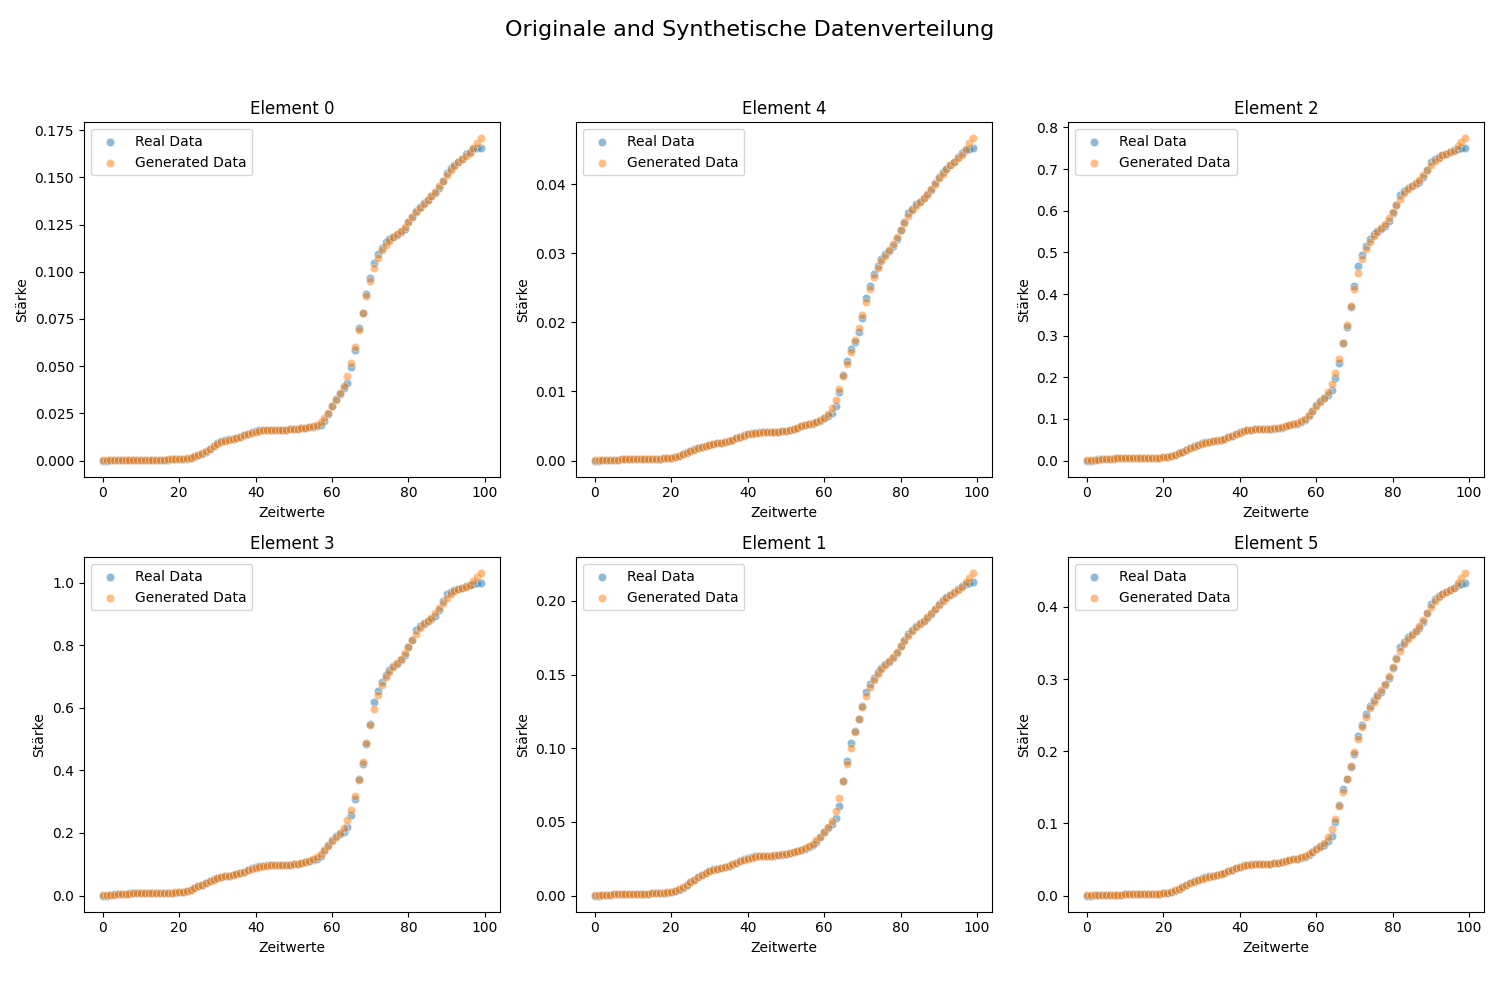
\includegraphics[width=\textwidth]{includes/figures/graphs/corona_histogram_tsa_compare.png}
        \caption{Übereinstimmung des SSA Algorihtmus mit den originalen Daten}
        \label{fig:graphs_ssa_histogram_compare}
    \end{minipage}
\end{figure}




\section{Vorhersagefähigkeiten der rekusiven Modelle}
Rekusive Modell haben einen weiteren Vorteil gegenüber den generattiven Modellen. Sie sind in der Lage auch einen die nächsten Werte vorherzusagen, was bei den generativen Modellen nicht möglich ist.
Hiermit bietet sich eine weitere Möglichkeit, neue Daten zu generieren.
Forcasts sind nicht so genau und variieren stark, abhängig von der Art der Daten. Sind die Muster ihnen bekannt, können sie recht gute vorhersagen treffen, bei komplexen Daten wie beispielsweise den Corona-Fallzahlen (Siehe Abbildung \ref{fig:corona_data})
ist dies aber nicht möglich, da sich hier noch kein Muster herausgebildet hat.


\begin{figure}[ht]
    \centering
    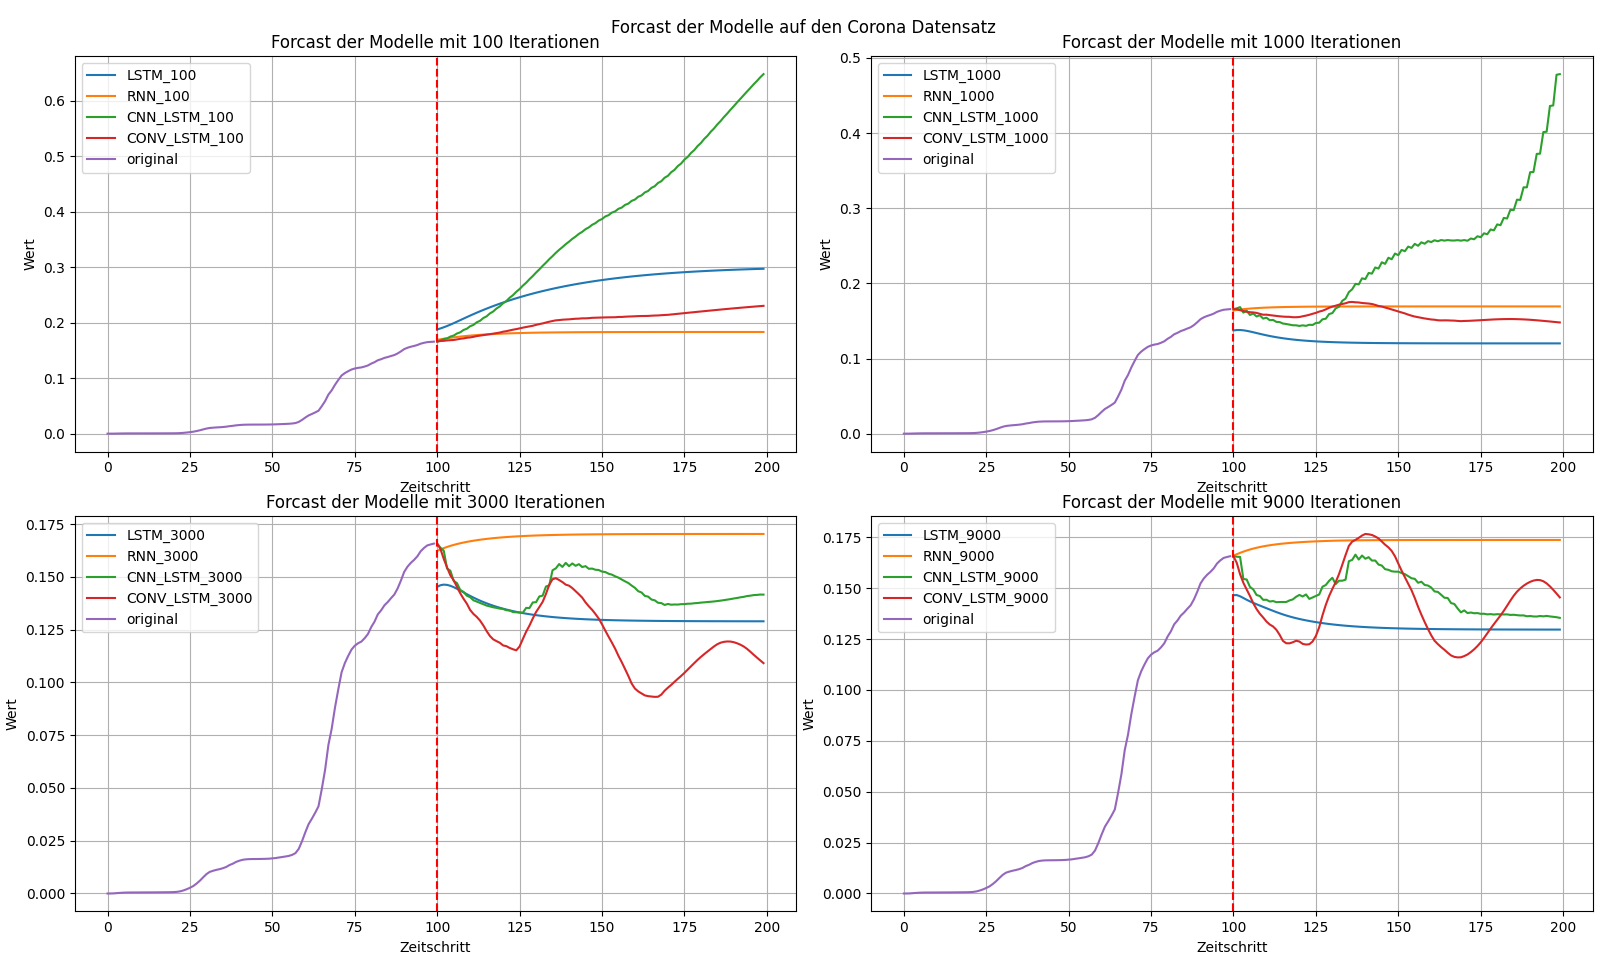
\includegraphics[width=1\textwidth]{includes/figures/graphs/forcast.png}
    \caption{Forcast der jeweiligen rekursiven Modelle}
    \label{fig:forcast_recursive_models}
\end{figure}







\section{Zusammenfassung}
Die gesammelten Daten zeigen ein gemischtes Bild. Wird grundsätzlich ein Vergleich zwischen \ac{ML} und \ac{TSA} angestrebt, so gewinnt immer der TSA Algorithmus, sollte es ein wunsch nach Performance und Resourcenverbrauch geben.
Hier können \ac{ML} Algorithmen einfach nicht mithalten.
Schaut man auf die \ac{MIA} Werte, so ist auch hier \ac{TSA} ein wenig dem \ac{ML} Modellen vorraus. Aber dies nur sofern viele Informationen verloren gehen.
GANs und CGANs sind sehr gut im erzeugen synthetischer Daten, neigen aber zu Überanpassungen, welches sie unvorhersehbar macht. Hier lässt aber eine direkte Korrelation zwischen der Komplexität der Daten und den entstehenden Resultaten herausfinden, wie in 
Tabelle \ref{tab:autocorrelation_coefficients} zu sehen ist. Die Sinus Daten trainieren deutlich schneller als die Wetterdaten und erreichen schneller bessere Werte, wie auch an den extern beigefügten Tabellen zu erkennen ist. Aber um eine definitive Aussage zu treffen, müsste man mehrere Datensätze ähnlicher Autokorrelationswerte testen.
Dies macht die gezielte Nutzung dieser Modelle nicht einfach. Um hier ein gewünschtes Ergebnis zu bekommen, muss im Notfall experimentiert werden.


\begin{figure}[ht]
    \centering
    \begin{minipage}{0.499\textwidth}
        \centering
        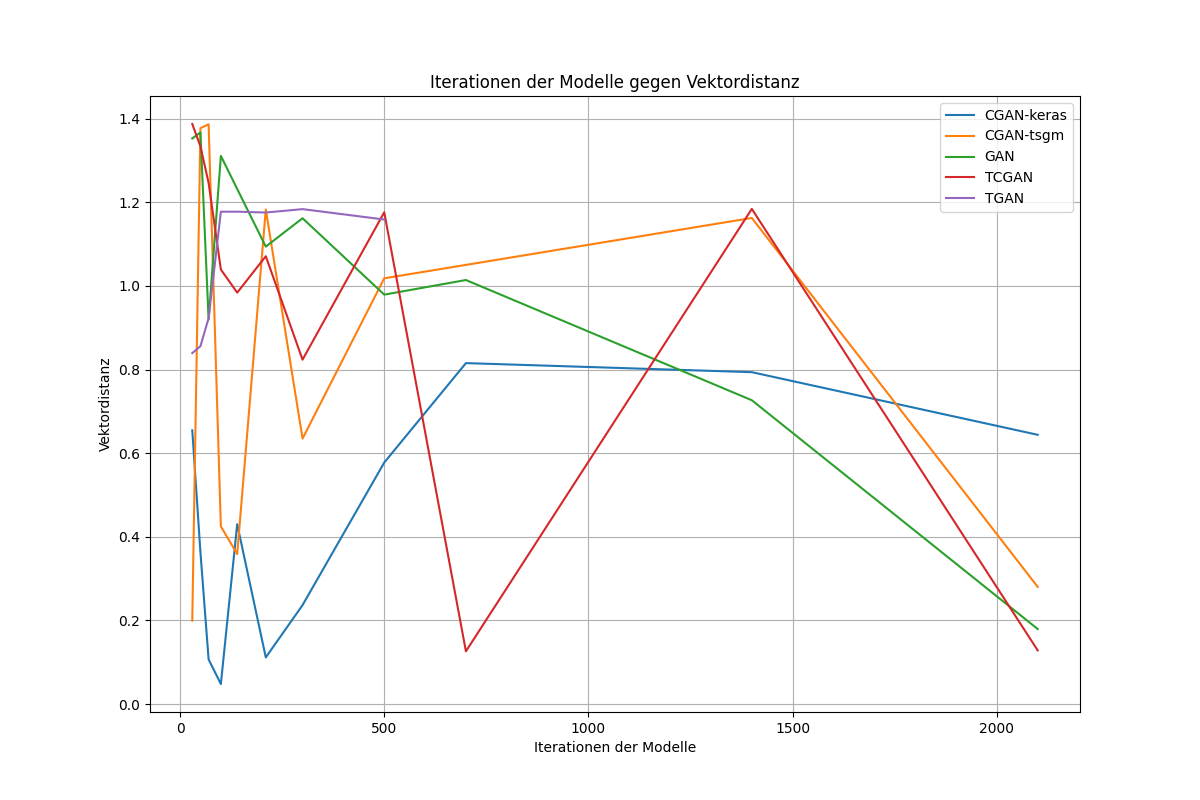
\includegraphics[width=\textwidth]{includes/figures/graphs/Iteration_attacker.similaritycorona.png}
        \caption{Vektordistanz zwischen den Lösungen und dem synthetischen Daten, Trainingsdaten: corona.csv}
        \label{fig:vect_dist_corona}
    \end{minipage}\hfill
    \begin{minipage}{0.499\textwidth}
        \centering
        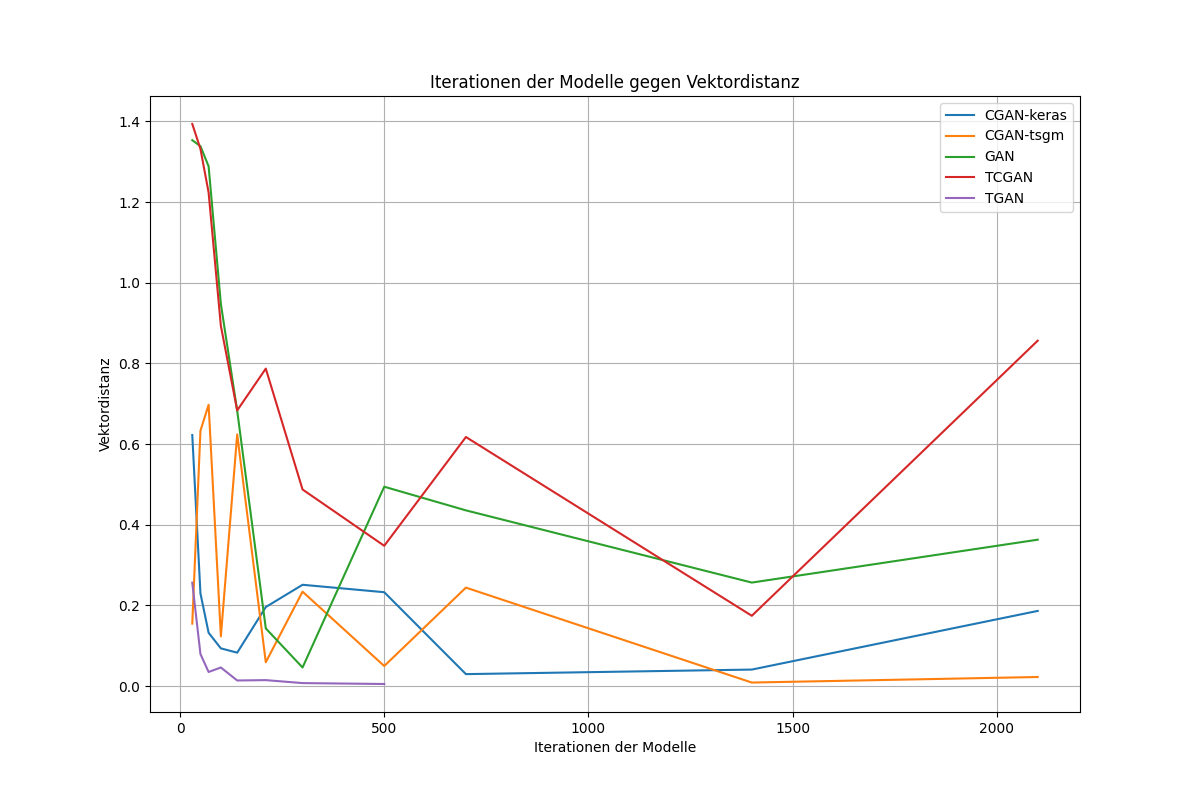
\includegraphics[width=\textwidth]{includes/figures/graphs/Iteration_attacker.similaritysinus.png}
        \caption{Vektordistanz zwischen den Lösungen und dem synthetischen Daten, Trainingsdaten: sinus.csv}
        \label{fig:vect_dist_sinus}
    \end{minipage}
\end{figure}

Dennoch zeigt das \ac{CGAN} eine durschnittlich deutlich bessere Performance als das normale GAN Modell.
Dies lässt sich auch an den Clustering Ergebnissen sehen. Diese sind separate im Anhang als 3D html Plots hinterlegt.
Vergleicht man die generativen Modelle mit den rekursiven Modellen, so muss eindeutig gesagt werden, dass diese eine deutlich besser Annäherung an die originalen Daten zeigen. Sie sind dabei auch deutlich schneller, benötigen also weniger Resourcen und sind einfacher zu trainieren.
Leider kommt durch die Annäherung auch eine geringe Privatsphäre, da die \ac{MIA} Metrik einen sehr niedrigen Wert zeigt.
Dann kommt dazu die uneindeutigkeit der Ergebnisse. Steigt die Komplexität, so steigt die Trainignszeit der Daten. Zu langes training kann aber zu Overfitting führen, eine zu kurze Trainingszeit zu einer schlechten Annäherung. Dies gibt dem Nutzer viel Kontrolle, aber dies nur durch ausgedehntes Testing oder einen guten loss Wert.
Hier wäre Erfahrung mit den Modellen aber wichtig.

Vergleicht man diese Werte mit den \ac{TSA} Algorithmen, so wirken diese primär erstmal deutlich attraktiver. Sie sind schneller, brauchen weniger Resourcen und sind auch recht flexibel. Selbst komplexe Zeitreihen können schnell approximiert werden.
Probleme wie Overfitting gibt es nicht. Underfitting lässt sich, jedenfalls beim Vorhandensein von genügend \ac{IMF}s, auch vermeiden, sogar steuern.
In Kombination mit dem Möglichkeiten des Frontends, welches, wie in Abbildung \ref{fig:tsa_trained_configuration} aus Sektion \ref{sec:reactTSA} hier direkt Veränderungen an der Konfiguration zulässt, ist dies ein sehr mächtiges Werkzeug, welches deutlich mehr Kontrolle an den Nutzer abgibt und ihn deutlich schneller zum Ziel führt.
Auch sind Modelle wie Amira, Cubic Spline oder das nicht implementierte Prophet in der Lage größere Datenmengen in kürzester Zeit zu verarbeiten.

Hier ist also eine Abwegung notwendig. Braucht man schnell die Daten, so sollte man auf jeden Fall zu Algorithem aus der Zeitreihenanalyse greifen. Hier erhält man direkt ein Ergebnis und kann dieses bei bedarf anpassen.
Machninelles Lernen wird bei Datenmengen interessant, welche groß und komplex sind, und bei denen meinen einen ungefähren Verlauf benötigt. 
Für komplexer Systeme, welche beispielsweise mit Außreißern klar kommen müssen, sind generative Modelle interessanter als TSA Algorithmen.

